% note-setup-borderless.tex
% fenglielie@qq.com 2025-07-10

\documentclass{article}
\usepackage{amsmath,amsthm,amsfonts,amssymb}
\usepackage{mathtools}
\usepackage{mathrsfs}
\usepackage{bm}
\usepackage{extarrows}
\usepackage[a4paper, margin=1in]{geometry}
\usepackage{float}
\usepackage{indentfirst}
\usepackage{anyfontsize}
\usepackage{booktabs,multirow,multicol}
\usepackage[shortlabels,inline]{enumitem}
\usepackage{appendix}

\usepackage[dvipsnames]{xcolor}
\usepackage{graphicx}
\graphicspath{
    {./figure/}{./figures/}{./image/}{./images/}{./graphic/}{./graphics/}{./picture/}{./pictures/}
}
\usepackage{subcaption}

\usepackage[ruled,linesnumbered,noline]{algorithm2e}
\usepackage{listings}
\lstdefinestyle{simpleStyle}{
    basicstyle=\ttfamily\small,
    breaklines=true,
    keywordstyle=\color{blue},
    identifierstyle=\color{black},
    stringstyle=\color{violet},
    commentstyle=\color[RGB]{34,139,34},
    showstringspaces=false,
    numbers=left,
    numbersep=2em,
    numberstyle=\footnotesize,
    frame=single,
    framesep=1em,
}
\lstset{style=simpleStyle}

\usepackage[colorlinks=true,linkcolor=,urlcolor=magenta,citecolor=violet]{hyperref}

\renewcommand*{\proofname}{\normalfont\bfseries Proof}

\usepackage{thmtools}
\usepackage{tikz}
\usepackage{tikz-cd}
\usepackage{tikz-3dplot}

%% define environments

\declaretheorem[style=plain, name=Theorem, numbered=yes, numberwithin=section]{theorem}
\declaretheorem[style=plain, name=Theorem, numbered=no]{theorem*}

\declaretheorem[style=plain, name=Proposition, numbered=yes, sibling=theorem]{proposition}
\declaretheorem[style=plain, name=Proposition, numbered=no]{proposition*}

\declaretheorem[style=plain, name=Corollary, numbered=yes, sibling=theorem]{corollary}
\declaretheorem[style=plain, name=Corollary, numbered=no]{corollary*}

\declaretheorem[style=plain, name=Lemma, numbered=yes, sibling=theorem]{lemma}
\declaretheorem[style=plain, name=Lemma, numbered=no]{lemma*}

\declaretheorem[style=plain, name=Claim, numbered=yes, sibling=theorem]{claim}
\declaretheorem[style=plain, name=Claim, numbered=no]{claim*}

\declaretheorem[style=definition, name=Definition, numbered=yes, numberwithin=section]{definition}
\declaretheorem[style=definition, name=Definition, numbered=no]{definition*}

\declaretheorem[style=definition, name=Example, numbered=yes, numberwithin=section]{example}
\declaretheorem[style=definition, name=Example, numbered=no]{example*}

\declaretheorem[style=definition, name=Problem, numbered=yes, numberwithin=section]{problem}
\declaretheorem[style=definition, name=Problem, numbered=no]{problem*}

\declaretheorem[style=remark, name=Remark, numbered=yes, numberwithin=section]{remark}
\declaretheorem[style=remark, name=Remark, numbered=no]{remark*}

\declaretheorem[style=remark, name=Note, numbered=yes, numberwithin=section]{note}
\declaretheorem[style=remark, name=Note, numbered=no]{note*}

\declaretheoremstyle[headfont=\bfseries, bodyfont=\normalfont, spaceabove=3pt, spacebelow=3pt, qed=\ensuremath{\square}]{solutionstyle}

\declaretheorem[style=solutionstyle, name=Solution, numbered=yes, numberwithin=section]{solution}
\declaretheorem[style=solutionstyle, name=Solution, numbered=no]{solution*}

\usepackage[most]{tcolorbox}

\newcommand{\newtcbenvironment}[2]{
    \tcolorboxenvironment{#1}{#2, enhanced, breakable, sharp corners, boxrule=0pt, colframe=white}
    \tcolorboxenvironment{#1*}{#2, enhanced, breakable, rounded corners, boxrule=0pt, colframe=white}
}

%% define styles

\newtcbenvironment{theorem}{colframe=RoyalPurple, colback=RoyalPurple!8}
\newtcbenvironment{proposition}{colframe=RoyalPurple, colback=RoyalPurple!8}
\newtcbenvironment{corollary}{colframe=NavyBlue, colback=SkyBlue!8}
\newtcbenvironment{lemma}{colframe=NavyBlue, colback=SkyBlue!8}
\newtcbenvironment{claim}{colframe=NavyBlue, colback=SkyBlue!8}

\newtcbenvironment{definition}{colframe=ForestGreen, colback=ForestGreen!5}
\newtcbenvironment{example}{colframe=RawSienna, colback=RawSienna!5}
\newtcbenvironment{problem}{colframe=WildStrawberry!30, colback=WildStrawberry!5}

\newtheorem{exercise}{Exercise}

%define short cut notation
\newcommand{\g}{\mathfrak{g}}
\newcommand{\h}{\mathfrak{h}}

\title{Riemann Surfaces}
\author{Zihan Ke}

\begin{document}
\maketitle
\section*{Introduction}
Riemann Surfaces is the one-dimensional complex manifold. Also, it can be described as the one-dimensional complex algeraic curves. I first encounter the concept of Riemann Surfaces in complex analysis.Later I found that Riemann Surfaces is not only an interesting object to learn itself. Since it cna be described as algebraic curves, it also provides a path to the study of algebraic geometry. I want to learn algebraic geometry and Riemann Surfaces is a good place to start. 
OUr goal in this note is to obtain Riemann-Roch theorem and its application.
\newpage
\tableofcontents 
\newpage

\section{Riemann Surfaces and complex \textbf{manifolds}.}
\subsection{Holomorphic functions in 1-variable}

Holomorphic functions are the central objects of study in complex analysis. They are functions defined on the complex plane that are ``complex differentiable,'' a condition that is far more restrictive and powerful than real differentiability.
\begin{definition}
A function $f: U \to \mathbb{C}$ on an open set $U \subseteq \mathbb{C}$ is said to be \textbf{holomorphic} if it is complex differentiable at every point $z_0 \in U$. This means the following limit, which defines the derivative $f'(z_0)$, exists:
\[ f'(z_0) = \lim_{h \to 0} \frac{f(z_0+h) - f(z_0)}{h} \]
\end{definition}
A key equivalent condition for holomorphicity is given by the \textbf{Cauchy-Riemann equations}. If we write $f$ in terms of its real and imaginary parts, $f(x+iy) = u(x,y) + iv(x,y)$, then $f$ is holomorphic if and only if $u$ and $v$ have continuous first partial derivatives that satisfy:
\[ \frac{\partial u}{\partial x} = \frac{\partial v}{\partial y} \quad \text{and} \quad \frac{\partial u}{\partial y} = -\frac{\partial v}{\partial x} \]
Holomorphic functions in one variable have several remarkable properties:
\begin{itemize}
    \item \textbf{Analyticity:} If a function is once complex differentiable, it is infinitely differentiable and can be represented by a convergent power series (Taylor series) in a neighborhood of every point.
    \item \textbf{Cauchy's Integral Formula:} The value of a holomorphic function inside a disk is completely determined by its values on the boundary circle.
    \item \textbf{Liouville's Theorem:} A holomorphic function on the entire complex plane (an ``entire'' function) that is bounded must be constant.
\end{itemize}

\subsection{Holomorphic functions in $n$-variables}

The theory of holomorphic functions in several complex variables, concerning functions $f: U \to \mathbb{C}$ on an open set $U \subseteq \mathbb{C}^n$, is a rich field with significant differences from the one-variable case.
\begin{definition}
A function $f(z_1, \dots, z_n)$ is said to be \textbf{holomorphic} if it is holomorphic with respect to each variable $z_j$ separately when all other variables are held constant. This means it must satisfy the Cauchy-Riemann equations for each variable $z_j = x_j + iy_j$.
\end{definition}
While this definition seems like a straightforward extension, the consequences are profound and lead to new phenomena not seen in one dimension:
\begin{itemize}
    \item \textbf{No Isolated Zeros:} In $\mathbb{C}$, the function $f(z)=z$ has an isolated zero at the origin. In $\mathbb{C}^n$ for $n \ge 2$, the zero set of a non-constant holomorphic function is never an isolated point. This is a consequence of \textbf{Hartogs's extension theorem}.
    \item \textbf{Domains of Holomorphy:} In one variable, for any open set, one can find a holomorphic function that cannot be extended analytically to any larger set. This is not true in higher dimensions. For example, any function holomorphic on a ``hollowed-out shell'' like $\{z \in \mathbb{C}^2 : 1 < ||z|| < 2\}$ can be automatically extended to the full ball $\{z \in \mathbb{C}^2 : ||z|| < 2\}$. This leads to the study of special domains called ``domains of holomorphy.''
\end{itemize}
These differences motivate the need for a more geometric viewpoint, which is provided by the theory of complex manifolds.

\subsection{Complex manifolds \& Riemann Surfaces.}

\begin{definition}
    Let $X$ be a \textbf{topological} space.
    \begin{enumerate}
        \item A $n$-dim \textbf{complex} chart on $X$ is a \textbf{homeomorphism}
        \[
        \phi : U \xrightarrow{\cong} V \subset \mathbb{C}^n \text{ open}
        \]
        \item Two such charts are compatible if
        $U_1 \cap U_2 = \emptyset$ or $\phi_2 \circ \phi_1^{-1} \big| \phi_1 (U_1 \cap U_2)$ is holomorphic
        \item A $n$-dim complex atlas $\mathcal{A}$ is a collection of pairwise compatible charts on $X$.
        \item Two such atlases on $X$ are equivalent if $\mathcal{A} \cup \mathcal{B}$ is an atlas.
        \item A $n$-dim $\mathbb{C}$ \textbf{manifold} is a topological space (is Hausdorff \& $2^{\text{nd}}$ countable) with an equivalence class of $n$-dim $\mathbb{C} \text{ atlases}$.
        \item A Riemann surface is a $1$-dim $\mathbb{C}$ \textbf{manifold}.
    \end{enumerate}
\end{definition}

\begin{exercise}
\begin{enumerate}
    \item Equivalence of atlases is an equivalence relation.
    \item $\exists$ unique maximal $\mathbb{C} \text{ atlas}$.
\end{enumerate}
\end{exercise}

\begin{remark}
    \begin{enumerate}[\upshape (i)]
        \item Refining an atlas doesn't change the complex structure.
        \item If $\phi : U \to V$ is a chart on Riemann Surface $X$.
        \[
        \alpha : V \xrightarrow{\wedge} W
        \]
        then $\alpha \circ \phi : U \to W$ is a chart compatible with $\phi$.
        \item An $n$-dimensional \textbf{manifold} is a $2n$-dimensional real smooth \textbf{manifold}.
    \end{enumerate}
\end{remark}

\subsection{Examples of Riemann Surfaces.}

\begin{example}
\begin{enumerate}
    The first example is a \textbf{Non-Examples:} 
    \item $X = \mathbb{R}^2 \times U \to V = \mathbb{C}$ for $i=1, 2$.
    \begin{align*}
        \phi_1 (x, y) &= x + iy \\
        \phi_2 (x, y) &= \frac{x+iy}{1+i dx^2 y^2}
    \end{align*}
    $\phi_1$ \& $\phi_2$ are not compatible.
    $\phi_2 \circ \phi_1^{-1} (z) = \frac{z}{1+|z|^2}$ not holomorphic.
    \item The complex plane $\mathbb{C}$.
    $X = \mathbb{R}^2$. with $\phi_1 : \mathbb{R}^2 \to \mathbb{C}$.
    \[
    (x, y) \mapsto x+iy
    \]
    is a Riemann Surface.
    \item The Riemann Sphere. $\mathbb{CP}^1$:
    $X = S^2 = \{ (x, y, z) \in \mathbb{R}^3 : x^2 + y^2 + z^2 = 1 \} \subset \mathbb{R}^3$.
    (the stereographic projection with some modifications)
\end{enumerate}
\end{example}

% The [!htbp] specifier suggests placement: here, top, bottom, or page of floats.
\begin{figure}[!h]
    % Centers the image horizontally on the page
    \centering
    
    % The main command to include the image.
    % 'width=0.8\textwidth' scales the image to 80% of the text width.
    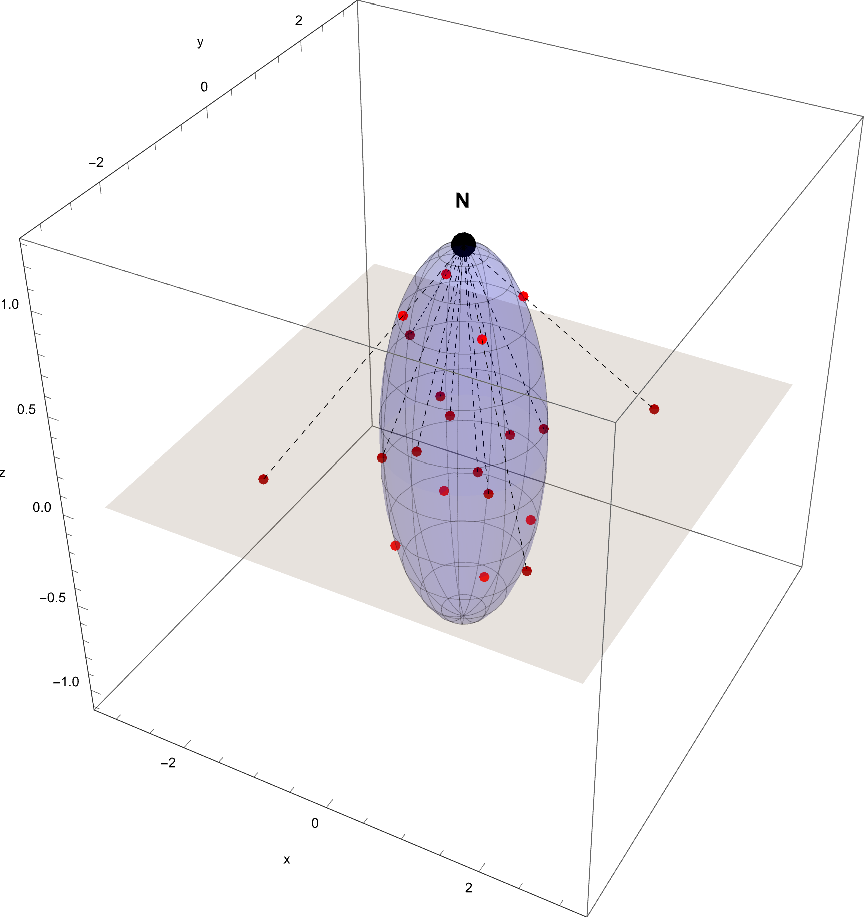
\includegraphics[width=0.5\textwidth]{stereograhic_projection.pdf}
    
    % Adds a caption below the image.
    \caption{Stereographic projection from the North Pole (N) of a sphere onto the plane $z=0$.}
    
    % Adds a label so you can reference the figure elsewhere using \ref{fig:stereo_proj}.
    \label{fig:stereo_proj}
\end{figure}

$S^2 \setminus \{ (0,0,1) \}$
\begin{align*}
    \phi_0 : U_0 &\longrightarrow V_0 = \mathbb{C} \\
    \parallel \\
    S^2 \setminus \{ (0, 0, 1) \} \\
    (x, y, w) &\longmapsto \frac{x+iy}{1-w} \quad \Rightarrow \quad \text{this is the stereographic projection}
\end{align*}
\begin{align*}
    \phi_{\infty} : U_{\infty} &\xrightarrow{\cong} V_{\infty} = \mathbb{C} \\
    \parallel \\
    S^2 \setminus \{ (0, 0, -1) \} \\
    (x, y, w) &\longmapsto \frac{x-iy}{1+w}
\end{align*}

\begin{exercise}
check these are charts.
\end{exercise} 

$\phi_0$ \& $\phi_{\infty}$ are compatible. On $U_0 \cap U_{\infty} = S^2 \setminus \{ (0,0,1), (0,0,-1) \}$, $\phi_0(U_0 \cap U_{\infty}) \subset \mathbb{C}^* \subset V_0$.

$$
\frac{1}{\phi_0(x, y, w)} = \frac{1-w}{x+iy} = \frac{(1-w)(x-iy)}{x^2+y^2} = \frac{(1-w)(x-iy)}{1-w^2} = \frac{x-iy}{1+w} = \phi_{\infty}(x, y, w)
$$

Thus,
$$
\phi_{\infty} \circ \phi_0^{-1} (z) = \frac{1}{z} \text{ on } \mathbb{C}^* = \phi_0 (U_0 \cap U_{\infty}) \subset \mathbb{C} = V_0.
$$
holomorphic

Hence, $\{ \phi_0, \phi_{\infty} \}$ are an atlas, and the corresponding Riemann Surface is called the **Riemann Sphere**.

\begin{enumerate}
    \item **Complex tori of dimension 1.**
    For $\omega_1, \omega_2 \in \mathbb{C}$ which are $\mathbb{R}$-linearly independent. consider the lattice $L = \mathbb{Z}\omega_1 + \mathbb{Z}\omega_2 = \{ n\omega_1 + m\omega_2 : n, m \in \mathbb{Z} \} \subset \mathbb{C}$.
    Let $X = \mathbb{C}/L$, with the quotient topology.
$$
\pi : \mathbb{C} \longrightarrow X = \mathbb{C}/L.
$$
$$
z \longmapsto [z] = z+L.
$$
Topologically $X$ is a torus.

Every $z \in \mathbb{C}$ is equivalent to a unique point in the
Fundamental domain.

\begin{center}
    % Placeholder for the fundamental domain parallelogram
    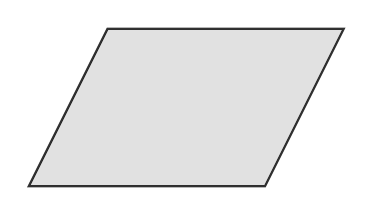
\begin{tikzpicture}
        \coordinate (A) at (0, 0);
        \coordinate (B) at (3, 0);
        \coordinate (C) at (4, 2);
        \coordinate (D) at (1, 2);
        \draw[thick, fill=gray!30, opacity=0.8] (A) -- (B) -- (C) -- (D) -- cycle;
    \end{tikzpicture}
\end{center}

Given $X = \mathbb{C}/L$, we construct an atlas using $\pi : \mathbb{C} \to \mathbb{C}/L$.

Pick $\varepsilon > 0$ s.t. $\forall p \in \mathbb{C}$, $B_{\varepsilon}(p)$ intersects each $[z]$ in at most one point.

Thus gives a homeomorphism
$$
\pi : B_{\varepsilon}(p) \xrightarrow{\cong} \pi(B_{\varepsilon}(p))
$$
$$
\text{with } \phi_p = \pi \big|_{B_{\varepsilon}(p)} : U_p \subset X
$$
where $U_p = \pi(B_{\varepsilon}(p))$.

\begin{claim*}
$$
\mathcal{A} = \{ \phi_p : U_p \to V_p \}_{p \in \mathbb{C}} \text{ is an atlas.}
$$
\end{claim*}
Compatibility of $\phi_p$ \& $\phi_q$:
Assume $U_{p, q} = U_p \cap U_q \neq \emptyset$.

The transition map is:
$$
T = \phi_q \circ \phi_p^{-1} : \phi_p(U_{p, q}) \longrightarrow \phi_q(U_{p, q})
$$
$T$ satisfies $\pi(T([z])) = \phi_p^{-1}([z]) = \pi([z])$ i.e., $T([z])-z \in L = \ker(\pi)$, which is constant.
$$
\Rightarrow T - \mathrm{id} \text{ is locally constant: locally } T - \mathrm{id} = w \in L.
$$
$$
T(z) = z + w \text{ is holomorphic}
$$
\end{enumerate}

\begin{center}
    % Placeholder for the diagram showing C mapping to X=torus
    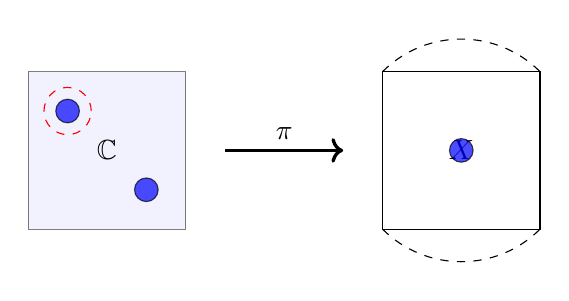
\begin{tikzpicture}
        % C plane (source)
        \draw[fill=blue!10, opacity=0.5] (-3, -0.5) rectangle (-1, 1.5);
        \node at (-2, 0.5) {$\mathbb{C}$};

        % X torus (target)
        \draw (1.5, -0.5) -- (3.5, -0.5) -- (3.5, 1.5) -- (1.5, 1.5) -- cycle;
        \draw[dashed] (1.5, 1.5) to[out=45, in=135] (3.5, 1.5);
        \draw[dashed] (1.5, -0.5) to[out=-45, in=-135] (3.5, -0.5);
        \node at (2.5, 0.5) {$X$};

        % Map pi
        \draw[->, very thick] (-0.5, 0.5) -- (1, 0.5) node[midway, above] {$\pi$};

        % Circles/points (covering map visualization)
        \draw[fill=blue, opacity=0.7] (-2.5, 1.0) circle (0.15);
        \draw[fill=blue, opacity=0.7] (-1.5, 0.0) circle (0.15);
        \draw[fill=blue, opacity=0.7] (2.5, 0.5) circle (0.15);
        \draw[dashed, red] (-2.5, 1.0) circle (0.3);
    \end{tikzpicture}
\end{center}

\subsection{Examples of complex manifolds}

\begin{example}[Complex Projective Plane]
$$
\mathbb{CP}^n = \{ \text{1-dimensional complex vector subspace in } \mathbb{C}^{n+1} \} = \mathbb{C}^{n+1} \setminus \{ 0 \} / \mathbb{C}^*.
$$
$$
\cong S^{2n+1} / S^1 \quad \text{ quotient topology.}
$$

Give $\mathbb{CP}^n$ the quotient topology.
$$
\pi : \mathbb{C}^{n+1} \setminus \{ 0 \} \longrightarrow \mathbb{CP}^n
$$
$$
(z_0, \dots, z_n) \longmapsto \pi(z_0, \dots, z_n) = [z_0 : z_1 : \dots : z_n].
$$
homogeneous coordinates.

\textbf{Atlases:}
Let
$$
U_i = \{ [z_0 : \dots : z_n] : z_i \neq 0 \} \subset \mathbb{CP}^n \quad \text{ open}
$$
The chart $\phi_i$ is given by:
$$
\phi_i : U_i \longrightarrow V_i = \mathbb{C}^n
$$
$$
[z_0 : \dots : z_n] \longmapsto \left( \frac{z_0}{z_i}, \frac{z_1}{z_i}, \dots, \widehat{\frac{z_i}{z_i}}, \dots, \frac{z_n}{z_i} \right)
$$
where $\widehat{\frac{z_i}{z_i}}$ denotes the omission of the $i$-th coordinate.
\end{example}

\section{Morphisms of complex manifolds \& meromorphic functions.}

\subsection{Morphisms of manifolds}

\begin{definition}
    Let $X$ \& $Y$ be complex \textbf{manifolds} of dimensions $n$ \& $m$ respectively.
    Let $W \subset X$ \& $W' \subset Y$ be open sets.
    \begin{enumerate}
        \item A continuous map $F: W \to W'$ is holomorphic at $p \in W$
        if $\exists$ charts $\phi : U \to V$ \& $\psi : W' \to V'$ s.t. $p \in U$
        \& $F(p) \in W'$, s.t. $\psi \circ F \circ \phi^{-1}$ is holo at $\phi(p)$.
        \item Biholomorphism.
    \end{enumerate}
\end{definition}

\begin{example}(Examples of Morphisms)
\begin{enumerate}
    \item A chart on a Riemann Surface $\phi : U \to V \subset \mathbb{C}$ on a Riemann Surface is a holomorphic function.
    \item Let $U \subset X$ for a Riemann Surface $X$. Then $U$ has a unique Riemann Surface structure s.t. the inclusion map $U \hookrightarrow X$ is holomorphic.
    \item Let $\mathbb{C}_{\infty} = \mathbb{C} \cup \{\infty\} \cong S^2 = U_0 \cup U_{\infty}$.
    Let $f$ be a holomorphic function on $\mathbb{C}$.
    Let $f_0 := f \circ \phi_0^{-1} : \mathbb{C} \to \mathbb{C}$.
    Let $f_{\infty} := f \circ \phi_{\infty}^{-1} : \mathbb{C} \to \mathbb{C}$.
On $\mathbb{C}^*$:
$$
f_{\infty}(w) = f \circ \phi_{\infty}^{-1}(w) = f \circ \phi_0^{-1} \circ \phi_0 \circ \phi_{\infty}^{-1}(w) = f_0 \left(\frac{1}{w}\right)
$$

This $f$ is holomorphic at $w \in \mathbb{C}_{\infty}$
$$
\iff f\left(\frac{1}{z}\right) \text{ is holomorphic at } 0
$$
$$
\Updownarrow \text{ Def}
$$
$$
f_{\infty}(w) \text{ is holomorphic at } 0 \iff f_0 \left(\frac{1}{w}\right) \text{ is holomorphic at } \infty
$$
 \item the quotient map $\pi: \mathbb{C}^n \to \mathbb{C}^n/L$ for a complex torus is holomorphic.
\end{enumerate}
\end{example}

subsection*{$\S$ 2.2. Properties of holomorphic maps of Riemann Surfaces.}

\begin{theorem}[The identity theorem] \label{thm:identity}
    Let $F, G: X \to Y$ be holomorphic maps of Riemann Surfaces s.t. $F$ \& $G$ agree on a subset of $X$ with an accumulation point.
    Then $F=G$.
\end{theorem}

\begin{theorem}[Local form of holomorphic maps] \label{thm:localform}
    Let $F: X \to Y$ be a non-constant holomorphic map of Riemann Surfaces.
    For $p \in X$ \& $q = F(p)$, $\exists$ unique $k \in \mathbb{Z}_{>0}$ and local charts $\phi : U \to V$ \& $\psi : U' \to V'$
    s.t. $F$ has local form
    $$
    \psi \circ F \circ \phi^{-1} : V \to V'
    $$
    $$
    z \mapsto z^k.
    $$
\end{theorem}

\begin{proof} 
    take any charts $\phi: U \to V \subset \mathbb{C}$ \& $\psi: U' \to V' \subset \mathbb{C}$.
$$
\begin{array}{ccc}
    X & \xrightarrow{F} & Y \\
    \downarrow{\phi} & & \downarrow{\psi} \\
    \mathbb{C} & \xrightarrow{f} & \mathbb{C}
\end{array}
\quad
\begin{array}{l}
    p \mapsto 0. \\
    q \mapsto 0.
\end{array}
$$

Shrink $V$ so $F(U) \subset U'$. Then $f = \psi \circ F \circ \phi^{-1} : V \to V'$
is holomorphic and $0 \mapsto 0$.

Define $k = \mathrm{ord}_0(f) \in \mathbb{Z}_{\ge 0}$. $\mathrm{ord}_0(f)$ is the order of vanishing of $f$
at $0 = \min \{ n \mid c_n \neq 0 \}$ where $f(z) = \sum_{n \ge 0} c_n z^n$ is
the Taylor expansion. $f(z) = z^k g(z)$, where $g(z)$ is non-zero.

Shrink $V$ so $g: V \to \mathbb{C}$ is non-zero and holomorphic.
Thus, $\exists$ holomorphic $k^{\text{th}}$ root $h: V \to \mathbb{C}$ of $g$
i.e., $(h(z))^k = g(z)$.

Thus $f(z) = z^k g(z) = (z h(z))^k$.

Let $\alpha : V \xrightarrow{\cong} \alpha(V)$ be biholomorphic
$$
z \mapsto z h(z) = w.
$$
Note $\alpha(0) = 0$, $\alpha'(0) = h(0) \neq 0$, then $\mathrm{ord}_0(\alpha) = 1$.

Now replace $\phi$ by $\alpha \circ \phi$.
$$
\psi \circ F \circ (\alpha \circ \phi)^{-1}(w) = \psi \circ F \circ \phi^{-1} \circ \alpha^{-1}(w)
$$
$$
= f(\alpha^{-1}(w)) = (\alpha^{-1}(w) h(\alpha^{-1}(w)))^k = w^k.
$$
Local form is $w \mapsto w^k$.
\end{proof}

\begin{exercise}
Show $k$ is independent of the choice of chart.
\end{exercise}
\begin{definition}
    The \textbf{multiplicity} of a non-constant holomorphic map $F: X \to Y$
    of Riemann Surfaces at $p \in X$ is the unique positive integer $k$ given by
    Theorem 2.2.
\end{definition}

We say $p$ is an \underline{unramified point} of $F$ if $\mathrm{mult}_p(F) = 1$.
$p$ is a \underline{ramified point} of $F$ if $\mathrm{mult}_p(F) > 1$.

$$
R(F) = \{ p \in X : \mathrm{mult}_p(F) > 1 \} \text{ ramification locus.}
$$
$$
B(F) = F(R(F)) \subset Y \text{ branch locus.}
$$

\begin{theorem}
    (Open mapping theorem) \label{thm:openmapping}
    A non-constant holomorphic map of Riemann Surfaces is an open mapping.
\end{theorem}

\textbf{Proof:} The local form $z \mapsto z^k$ is open
("maps circle to circle").

\begin{theorem}
    (Biholomorphic maps are biholomorphisms) \label{thm:biholo}
    The inverse of a bijective holomorphic map of Riemann Surfaces is holomorphic
    (since $F$ is an open mapping).
\end{theorem}

\begin{theorem}
(Discreteness of preimages)
Let $F: X \to Y$ non constant map of RS. Then $\forall q \in Y$.
the preimage $F^{-1}(q)$ is discrete in $X$.
(\textcolor{red}{If $X$ is compact then $F^{-1}(q)$ is finite})
\end{theorem}

\begin{proof}
$F$ follows as a holomorphic map of the complex plane are discrete.
\end{proof}

\begin{theorem}
(Surjectivity of non-constant holomorphic map from compact RS)
Let $F: X \to Y$ a non-constant holomorphic map of RS with $X$ compact.
Then $F$ is surjective and $Y$ is compact.
\end{theorem}

\begin{proof}
Open mapping theorem $\implies F(X) \subset Y$ is open
$F$ continuous and $X$ compact $\implies F(X)$ compact hence closed (and $Y$ hausdorff) $\square$.
\end{proof}

\begin{corollary}
Every holomorphic function on a compact Riemann Surface ($\mathbf{RS}$) is constant.
\end{corollary}
\textbf{Proof:}
Let $f: X \to \mathbb{C}$ be a non-constant holomorphic function.
Then $f$ is constant.
\hfill $\square$

\begin{theorem} [Riemann's extension theorem] 
Let $X$ be a $\mathbf{RS}$, $p \in U \subset_{\text{open}} X$. If $f: U \setminus \{p\} \to \mathbb{C}$ is holomorphic and bounded in a punctured neighborhood of $p$, then $f$ extends to a holomorphic function on $U$.
\end{theorem}
\textbf{Proof:}
Follows from complex analysis using charts.
\hfill $\square$

\begin{theorem} [Maximum principle] 
Let $f: X \to \mathbb{C}$ be a non-constant holomorphic function on a $\mathbf{RS}$ $X$.
Then $|f|$ has no local maximum.
\end{theorem}

\subsection{Meromorphic functions on Riemann Surfaces}

\begin{definition}
Let $X$ be a $\mathbf{RS}$ and $p \in W \subset_{\text{open}} X$. If $f: W \setminus \{p\} \to \mathbb{C}$ is holomorphic, we say that $p$ is a
$$
\left\{
\begin{array}{ll}
\text{removable singularity} & \\
\text{pole} &  \\
\text{essential singularity} & 
\end{array}
\right\}
\text{ if } \exists \text{ chart } \phi: U \to V , \text{ s.t. } \phi(p) \text{ is a }
\left\{
\begin{array}{l}
\text{removable singularity} \\
\text{pole} \\
\text{essential singularity}
\end{array}
\right\}
$$
We say $f$ is **meromorphic** at $p$ if $p$ is a **non-essential singularity**.

If $S \subset W \subset_{\text{open}} X$ and $f: W \setminus S \to \mathbb{C}$ is holomorphic, we say $f$ is **meromorphic** on $W$ if it is **meromorphic** at each $p \in S$.
\end{definition}

\textbf{Notation}
Let $U \subset_{\text{open}} X$.
\begin{itemize}
    \item $\mathcal{O}_X(U) = \{f: U \to \mathbb{C} \mid f \text{ is holomorphic}\}$
    \item $\mathcal{M}_X(U) = \{f: U \setminus S \to \mathbb{C} \mid f \text{ is meromorphic on } U\}$
\end{itemize}

\begin{lemma}
\begin{enumerate}[i)]
    \item The above definition is independent of the choice of chart.
    \item $\mathcal{O}(X) = \mathcal{O}_X(X)$ is a $\mathbb{C}$-algebra.
    \item $\mathcal{M}(X) = \mathcal{M}_X(X)$ is a field, called the **function field of $X$**.
    \item $\mathcal{M}(X) = \text{Frac}(\mathcal{O}(X))$.
    \item $p$ has a
    $$
    \left\{
    \begin{array}{l}
    \text{removable singularity} \\
    \text{pole} \\
    \text{essential singularity}
    \end{array}
    \right\} \text{ at } p \text{ if }
    \left\{
    \begin{array}{l}
    |f| \text{ is bounded in a neighborhood of } p \\
    \lim_{z \to p} |f(z)| = \infty \\
    \lim_{z \to p} f(z) \text{ doesn't exist}
    \end{array}
    \right\}
    $$
\end{enumerate}
\end{lemma}

\subsection{Laurent Expansions \& Orders of Singularities}
Let $f: W \setminus \{p\} \to \mathbb{C}$ be a holomorphic function with $p \in W \subset_{\text{open}} X$, where $X$ is a **Riemann Surface**.
Let $\phi: U \to V$ be a chart on $X$, such that $\phi(p) = 0$.
Then $f \circ \phi^{-1}: V \setminus \{0\} \to \mathbb{C}$ is holomorphic and has a Laurent expansion at $0$.
$$
f \circ \phi^{-1}(z) = \sum_{n = -\omega}^{\infty} c_n z^n \quad \text{(\textbf{Note}: This depends on the choice of chart.)}
$$

\begin{definition}
The **order of $f$** is defined as:
$$
\text{ord}_p(f) := \text{ord}_0(f \circ \phi^{-1}) = \min \{n \in \mathbb{Z} \mid c_n \neq 0\}
$$
If $f(z) = 0$ for all $z$, then $\text{ord}_p(0) = \infty$.
\end{definition}

\begin{lemma}
\begin{enumerate}[i)]
    \item $\text{ord}_p(f)$ is independent of the chart $\phi$ centered at $p$.
    \item $X$ is a
    $$
    \left\{
    \begin{array}{l}
    \text{removable singularity} \\
    \text{pole} \\
    \text{essential singularity}
    \end{array}
    \right\} \text{ of } f \text{ if } \text{ord}_p(f) =
    \left\{
    \begin{array}{l}
    \geq 0 \\
    -m, \quad m > 0 \quad \text{(i.e., } < 0 \text{)} \\
    -\infty
    \end{array}
    \right\}
    $$
    \item $\text{ord}_p(f^{-1}) = -\text{ord}_p(f)$.
    \item $\text{ord}_p(f g) = \text{ord}_p(f) + \text{ord}_p(g)$.
    \item $\text{ord}_p(f+g) \geq \min \{ \text{ord}_p(f), \text{ord}_p(g) \}$.
\end{enumerate}
\end{lemma}

\begin{example}
The map $\exp: \mathbb{C} \to \mathbb{C}$ is holomorphic on $\mathbb{C}$. Is it holomorphic or meromorphic on $\mathbb{C}_{\infty}$?
Consider $w=1/z$. For $f: \mathbb{C}_{\infty} \setminus \{0\} \to \mathbb{C}$ we have $\text{ord}_{\infty}(f) = \text{ord}_0(f(1/z))$.
Thus, $\exp(w)$ has an essential singularity at $w=0$, so $\exp$ is not meromorphic on $\mathbb{C}_{\infty}$.
\end{example}

\begin{example} [Meromorphic functions on $\mathbb{C}_{\infty}$]
Let $z=\phi_0: U_0 \to V_0 = \mathbb{C}$. $\text{ord}_0(z) = -1$ .
Let $P, Q \in \mathbb{C}[z]$ with $Q \not\equiv 0$. We claim $f(z) = P(z)/Q(z) \in \mathcal{M}(\mathbb{C}_{\infty})$.
We know $f \in \mathcal{M}(\mathbb{C})$: what about at $\infty$?
Let $f(z) = \lambda \prod_{i} (z-a_i)^{k_i}$, where $a_i \in \mathbb{C}$ and $k_i \in \mathbb{Z}$. $x \in \mathbb{C}$.
$f(z)$ is meromorphic at $\infty$ if $f(1/z)$ is meromorphic at $0$.
$$
f(1/z) =\lambda \prod_{i} (1/z - a_i)^{k_i} = \lambda z^{-\sum k_i} \prod_{i}  (1 - a_i z)^{k_i}
$$
$$
\text{ord}_{\infty}(f) =
\left\{
\begin{array}{ll}
-\sum k_i & p=\infty \\
k_i & p=a_i \\
0 & \text{otherwise}
\end{array}
\right.
\quad \text{Note: } \sum_{p \in \mathbb{C}_{\infty}} \text{ord}_p(f) = 0.
$$
\end{example}

\begin{theorem} [Meromorphic functions as holomorphic maps to $\mathbb{C}_{\infty}$] 
For a **Riemann Surface** $X$, there is a 1-1 correspondence:
$$
\mathcal{M}(X) = \{ \text{meromorphic functions on } X \} \longleftrightarrow \{ \text{holomorphic maps } F: X \to \mathbb{C}_{\infty} \mid F \not \equiv \infty \}
$$
The correspondence is given by:
$$
f \longmapsto F: X \to \mathbb{C}_{\infty}, \quad F(x) =
\left\{
\begin{array}{ll}
f(x), & x \notin \text{Pole}(f) \\
\infty, & x \in \text{Pole}(f)
\end{array}
\right.
$$
$$
f = \phi_{\infty} \circ F \mid_{F^{-1}(\mathbb{C})} \longleftarrow F: X \to \mathbb{C}_{\infty}.
$$
and $f(x)=\infty$ if $F(x)=\infty$.
\end{theorem}

\begin{proof}
The map $F$ associated to $f \in \mathcal{M}(X)$ is holomorphic on $X \setminus \text{Pole}(f)$.
\textbf{We want to show:} $F$ is holomorphic at each $p \in \text{Pole}(f)$.
$f$ has a pole at $p \iff f \circ \psi^{-1}$ has a pole at $\psi(p)=0$ (by definition).\\
$\iff \phi_{\infty} \circ F \circ \psi^{-1} = \frac{1}{f \circ \phi^{-1}} \text{ has a zero at } \psi(p) = 0.$
This means $F$ is holomorphic at $p$ (by definition of holomorphicity for a map to $\mathbb{C}_{\infty}$).
\end{proof}

\begin{lemma} [Relating the order of $f \in \mathcal{M}(X)$ and the multiplicity of the corresponding map $F: X \to \mathbb{C}_{\infty}$]
For $f \in \mathcal{M}(X)$ non-constant, and $F: X \to \mathbb{C}_{\infty}$ the corresponding holomorphic map at $p \in X$:
\begin{enumerate}[i)]
    \item If $f(p)=0$, then $\text{mult}_p(F) = \text{ord}_p(f)$.
    \item If $f(p)=\infty$, then $\text{mult}_p(F) = -\text{ord}_p(f)$.
    \item Otherwise, $\text{mult}_p(F) = \text{ord}_p(f - f(p))$.
\end{enumerate}
\end{lemma}

\begin{theorem} [Meromorphic functions on $\mathbb{C}_{\infty}$] 
$$\mathcal{M}(\mathbb{C}_{\infty})=\mathbb{C}(z)$$
\end{theorem}

\textbf{Proof:}
We've seen $\mathbb{C}(z) \subset \mathcal{M}(\mathbb{C}_{\infty})$. Let $f \in \mathcal{M}(\mathbb{C}_{\infty})$.
Let $p_1, p_2, \dots, p_n$ be the zeros of $f$ in $\mathbb{C} \subset \mathbb{C}_{\infty}$.
Let $g(z) := \prod_{i=1}^n (z-p_i)^{r_i}$, where $r_i = \text{ord}_{p_i}(f) \in \mathbb{Z}$.
(Note that $g(z) \in \mathbb{C}(z)$).
By construction, $\text{ord}_p(f) = \text{ord}_p(g)$ for all $p \in \mathbb{C}$. Then $h = f/g \in \mathcal{M}(\mathbb{C}_{\infty})$ has no zeros and no poles in $\mathbb{C}$.

Let $h(z) = \sum c_n z^n$ be the Taylor expansion of $h$ at $0 \in \mathbb{C}$.
Let $w = 1/z$ be a local coordinate at $\infty \in \mathbb{C}_{\infty}$. Then
$$
h(w) = \sum c_n w^{-n}
$$
is the Laurent expansion of $h$ at $\infty$.
Since $h$ is meromorphic at $\infty$, then $h(z) = \sum_{n=0}^m c_n z^n \in \mathbb{C}[z]$ (polynomial).
If $\deg(h) > 0$, then $h$ has a zero in $\mathbb{C}$. Thus $h(z) = \lambda$, a constant.
And $f = \lambda g \in \mathbb{C}(z)$.
\hfill $\square$

\begin{corollary}
For $f \in \mathcal{M}(\mathbb{C}_{\infty})$, $\sum_{p \in \mathbb{C}_{\infty}} \text{ord}_p(f) = 0$.
\end{corollary}

\subsection{The degree of a holomorphic map}

\begin{theorem} \label{degree of holo map between copt rs}
Let $F: X \to Y$ be a non-constant holomorphic map of compact **Riemann Surfaces**.
For $q \in Y$, the quantity $\text{deg}_q(F) = \sum_{p \in F^{-1}(q)} \text{mult}_p(F)$ is independent of $q$.
\end{theorem}

\begin{definition}
The **degree of $F$** is $\deg(F) = \deg_q(F)$ for any $q \in Y$.
\end{definition}

\begin{proof}
For $q \in Y$, take $F^{-1}(q) = \{p_1, p_2, \dots, p_s\}$ and let $k_i = \text{mult}_{p_i}(F)$.
By Theorem 2.2, $\exists$ local normal forms at each $p_i$, i.e.,
$\exists$ charts $\phi_i: U_i \to V_i$ on $X$ and $\psi: U_i' \to V_i'$ on $Y$,
such that $F(U_i) \subset U_i'$, $p_i \to 0$, $q \to 0$,
and $\psi \circ F \circ \phi_i^{-1}(z) = z^{k_i}$. Assume the $U_i$ are pairwise disjoint.
\begin{claim*}
$\exists$ open neighborhood $W$ of $q$ in $Y$ such that $F^{-1}(W) \subset \bigcup_{i} U_i$.
\end{claim*}
\textbf{Proof of Claim:}
Let $\overline{W}$ be an open neighborhood of $q$, $\overline{W} = \{q\} \cup \text{something else}$.
Let $W$ be an open neighborhood of $q$ such that $W \cap F(X \setminus \bigcup_i U_i) = \emptyset$.
Thus $F^{-1}(W) \cap (X \setminus \bigcup_i U_i) = \emptyset$.
Since $X$ is compact, $F(X \setminus \bigcup_i U_i)$ is compact.
$\exists$ an open neighborhood $W_i$ of $q$ in $Y$ such that $F^{-1}(W_i) \cap (X \setminus U_i) = \emptyset$.Let $W = \bigcap_{i=1}^s W_i$, which is an open neighborhood of $q$. Then $F^{-1}(W) \subset \bigcup_{i=1}^s U_i$. $\square$

For any $q' \in W$, we have $\deg_{q'}(F) = \deg_q(F)$.
This is because, for $q' \in W$, $F^{-1}(q') \cap U_i$ consists of $k_i$ points of multiplicity 1.
Hence $\deg_q(F)$ is locally constant, and as $Y$ is connected, $\deg_q(F)$ is constant.
\end{proof}

\begin{remark}
Let $f: X \to \mathbb{C}$. If $f$ is locally constant and $X$ is connected,
then $f$ is a constant.
\end{remark}

\begin{proof}
Take $p \in X$. $\exists U_p \subset X$ such that $f|_{U_p}$ is a constant $f(p)$.
Consider $\mathcal{O} = \{x \in X \mid f(x) = f(p)\}$.
\begin{enumerate}
    \item $\mathcal{O}$ is open since $f$ is locally constant.
    \item $\mathcal{O}$ is closed since $f$ is locally constant.
\end{enumerate}
If $y \in X \setminus \mathcal{O}$, then $f(y) \neq f(p)$. Then $\exists U_y$ such that $U_y \subset X \setminus \mathcal{O}$.
Since $X$ is connected and $\mathcal{O}$ is non-empty (as $p \in \mathcal{O}$) and is both open and closed, we must have $\mathcal{O} = X$.
Thus $f$ is constant.
\end{proof}

\begin{remark}
\begin{enumerate}
    \item At a ramification point $p$, $F$ looks locally like $\mathbb{C} \to \mathbb{C}, z \mapsto z^k$.
    \item $F|_{X \setminus R(F)}: X \setminus R(F) \to Y \setminus B(F)$ is a $d$-sheeted covering, where $d = \deg(F)$.
\end{enumerate}
\end{remark}

\begin{corollary}
\begin{enumerate}[i)]
    \item If $F$ is a degree 1 non-constant holomorphic map of compact **Riemann Surfaces** ($\mathbf{RS}$), then $F$ is a **biholomorphism** (surjectivity + injectivity).
    \item If $X$ is compact and has a meromorphic function with a single simple pole, then $X \cong \mathbb{C}_{\infty}$.
\end{enumerate}
\end{corollary}

\begin{proof}
    \begin{exercise}
        
    \end{exercise}
\end{proof}

\begin{corollary}
$\mathbb{C}\mathbb{P}^1 \cong \mathbb{C}_{\infty}$.
\end{corollary}

\begin{corollary}
Let $X$ be a compact **Riemann Surface** ($\mathbf{RS}$) and $f \in \mathcal{M}(X)$ non-constant.
Then $\sum_{p \in X} \text{ord}_p(f) = 0$.
\end{corollary}

\begin{proof}
Let $F: X \to \mathbb{C}_{\infty}$ be the associated holomorphic map.
We know that:
$$
\sum_{p \in X} \text{ord}_p(f) = \sum_{p \in \text{Zero}(f)} \text{ord}_p(f) + \sum_{p \in \text{Pole}(f)} \text{ord}_p(f)
$$
We use the relationship between order and multiplicity
$$
\sum_{p \in \text{Zero}(f)} \text{ord}_p(f) = \sum_{p \in F^{-1}(0)} \text{mult}_p(F)
$$
And
$$
\sum_{p \in \text{Pole}(f)} \text{ord}_p(f) = \sum_{p \in F^{-1}(\infty)} (-\text{mult}_p(F)) = -\sum_{p \in F^{-1}(\infty)} \text{mult}_p(F)
$$
Substituting these back:
$$
\sum_{p \in X} \text{ord}_p(f) = \sum_{p \in F^{-1}(0)} \text{mult}_p(F) - \sum_{p \in F^{-1}(\infty)} \text{mult}_p(F)
$$
Since $\sum_{p \in F^{-1}(q)} \text{mult}_p(F) = \deg(F)$ for any $q \in \mathbb{C}_{\infty}$:
$$
= \deg(F) - \deg(F) = 0.
$$
\end{proof}

\subsection{Germs of holomorphic functions}

\begin{definition}
For a complex manifold $X$ and $p \in X$, we define the ring of germs of holomorphic functions at $p$:
$$
\mathcal{O}_{X, p} = \left\{ (U, f) \mid U \text{ is an open neighborhood of } p, f: U \to \mathbb{C} \text{ is holomorphic} \right\} / \sim
$$
where $\sim$ is the equivalence relation defined by:
$$
(U, f) \sim (V, g) \iff \exists \text{ a neighborhood } W \text{ of } p \text{ s.t. } f|_W = g|_W
$$
The equivalence class $[(U, f)]$ is called the **germ of $f$ at $p$**.
\end{definition}

\begin{remark}
\begin{enumerate}
    \item $\mathcal{O}_{X, p}$ is a ring whose non-invertible elements form an ideal.
    \item The maximal ideal $\mathfrak{m}_p$ is given by:
    $$
    \mathfrak{m}_p = \{ [(U, f)] \mid f(p) = 0 \}. \quad (\text{germs vanishing at } p)
    $$
    This is the kernel of the evaluation map:
    $$
    \text{ker}(\text{ev}_p: \mathcal{O}_{X, p} \to \mathbb{C}).
    $$
    Thus $\mathcal{O}_{X, p} / \mathfrak{m}_p \cong \mathbb{C}$. This means $\mathfrak{m}_p$ is a **maximal ideal** (local ring).
\end{enumerate}
\end{remark}

\begin{example}
\begin{enumerate}
    \item $\mathcal{O}_{\mathbb{C}^n, 0} \cong \mathbb{C} \{x_1, \dots, x_n\}$.
    $$
    [(U, f)] \mapsto \text{Taylor expansion of } f \text{ at } 0.
    $$
    \item If $X$ is an $n$-dimensional complex manifold and $p \in X$, then a local chart $\phi: U \to V$, centered at $p$, induces an isomorphism:
    $$
    \phi^*: \mathcal{O}_{\mathbb{C}^n, 0} \to \mathcal{O}_{X, p}
    $$
    which maps the germ $[(V, \psi)]$ to the germ $[(U, \psi \circ \phi)]$.
\end{enumerate}
\end{example}

\subsection{$\mathcal{O}_{X, p}$ for a Riemann Surface}
The order of a **holomorphic** function at $p$ descends to a map
$$
\text{ord}_p: \mathcal{O}_{X, p} \to \mathbb{N} \cup \{\infty\} \text{ satisfying}
$$

\begin{enumerate}
    \setcounter{enumi}{2} % Continue from the previous list on the previous page
    \item $\text{ord}_p(f) = \infty \iff f \equiv 0$.
    \item $\text{ord}_p(f g) = \text{ord}_p(f) + \text{ord}_p(g)$.
    \item $\text{ord}_p(f+g) \geq \min \{\text{ord}_p(f), \text{ord}_p(g)\}$.
\end{enumerate}
This is known as a **discrete valuation**.

We can extend $\text{ord}_p$ to $\text{Frac}(\mathcal{O}_{X, p})$ by $\text{ord}_p(f/g) = \text{ord}_p(f) - \text{ord}_p(g)$.

\begin{lemma}
For a **Riemann Surface** $X$, $\mathcal{O}_{X, p}$ is a **Discrete Valuation Ring** ($\mathbf{DVR}$) with valuation given by $\text{ord}_p: \text{Frac}(\mathcal{O}_{X, p}) \to \mathbb{Z} \cup \{\infty\}$.
The **uniformizer** (element with valuation 1) is given by a local chart centered at $p$.
\end{lemma}

\subsection{Jacobians and the implicit function theorem}

\begin{definition}
The complex Jacobian of a holomorphic map $f: \mathbb{C}^n \to \mathbb{C}^m$ at $p \in \mathbb{C}^n$ is
$$
J_{\mathbb{C}} f(p) := \left( \frac{\partial f_j}{\partial z_k} (p) \right)_{j, k} = \begin{pmatrix}
\frac{\partial f_1}{\partial z_1} (p) & \cdots & \frac{\partial f_1}{\partial z_n} (p) \\
\vdots & \ddots & \vdots \\
\frac{\partial f_m}{\partial z_1} (p) & \cdots & \frac{\partial f_m}{\partial z_n} (p)
\end{pmatrix} \in M_{m \times n} (\mathbb{C})
$$
We say $p$ is a \textbf{regular point} of $f$ if $J_{\mathbb{C}} f(p): \mathbb{C}^n \to \mathbb{C}^m$ is surjective.
We say $q \in \mathbb{C}^m$ is a \textbf{regular value} of $f$ if all of its preimages are regular points.
\end{definition}

\begin{example}
If $n=m=1$, then $J_{\mathbb{C}} f(p) = \left( \frac{\partial f}{\partial z} (p) \right)$.
\end{example}

\textbf{Relationship with the Real Jacobian}\\
Consider $f: \mathbb{C}^n \to \mathbb{C}^m$ real differentiable.
$$
\begin{array}{ccc}
\mathbb{C}^n & \to & \mathbb{C}^m \\
\mathbb{R}^{2n} & & \mathbb{R}^{2m}
\end{array}
$$

$$
J_{\mathbb{R}} f(p) = \begin{pmatrix}
\left( \frac{\partial u_j}{\partial x_k} (p) \right)_{j, k} & \left( \frac{\partial u_j}{\partial y_k} (p) \right)_{j, k} \\
\left( \frac{\partial v_j}{\partial x_k} (p) \right)_{j, k} & \left( \frac{\partial v_j}{\partial y_k} (p) \right)_{j, k}
\end{pmatrix} \in M_{2m \times 2n} (\mathbb{R})
$$
If $f$ is holomorphic at $p$:
$$
\begin{pmatrix}
\left( \frac{\partial u_j}{\partial x_k} (p) \right)_{j, k} & \left( \frac{\partial u_j}{\partial y_k} (p) \right)_{j, k} \\
- \left( \frac{\partial u_j}{\partial y_k} (p) \right)_{j, k} & \left( \frac{\partial u_j}{\partial x_k} (p) \right)_{j, k}
\end{pmatrix}
$$

Extend coordinates from $\mathbb{R}$ to $\mathbb{C}$ and consider the change of basis:
$$
\frac{\partial}{\partial \bar{z}_k} \quad \frac{\partial}{\partial z_k}
$$
$$
\frac{\partial}{\partial z_k} = \frac{1}{2} \left( \frac{\partial}{\partial x_k} - i \frac{\partial}{\partial y_k} \right) \quad \text{and} \quad \frac{\partial}{\partial \bar{z}_k} = \frac{1}{2} \left( \frac{\partial}{\partial x_k} + i \frac{\partial}{\partial y_k} \right)
$$
In the language of manifolds, $J_{\mathbb{R}}$ is written under the basis $\frac{\partial}{\partial x_k}$ and $\frac{\partial}{\partial y_k}$.
Now we do change of basis to $\frac{\partial}{\partial z_k}$ and $\frac{\partial}{\partial \bar{z}_k}$.

$$
\left[ \frac{\partial}{\partial x_1}, \ldots, \frac{\partial}{\partial x_n}, \frac{\partial}{\partial y_1}, \ldots, \frac{\partial}{\partial y_n} \right] A = T \left[ \frac{\partial}{\partial x_1}, \ldots, \frac{\partial}{\partial x_n}, \frac{\partial}{\partial y_1}, \ldots, \frac{\partial}{\partial y_n} \right] \quad (\ast)
$$
$$
\left[ \frac{\partial}{\partial z_1}, \ldots, \frac{\partial}{\partial z_n}, \frac{\partial}{\partial \bar{z}_1}, \ldots, \frac{\partial}{\partial \bar{z}_n} \right] B = T \left[ \frac{\partial}{\partial z_1}, \ldots, \frac{\partial}{\partial \bar{z}_n} \right] \quad (\ast\ast)
$$
Also note that
$$
\left[ \frac{\partial}{\partial z_1}, \ldots, \frac{\partial}{\partial z_n}, \frac{\partial}{\partial \bar{z}_1}, \ldots, \frac{\partial}{\partial \bar{z}_n} \right] = \left[ \frac{\partial}{\partial x_1}, \ldots, \frac{\partial}{\partial x_n}, \frac{\partial}{\partial y_1}, \ldots, \frac{\partial}{\partial y_n} \right] P
$$
$$
P = \frac{1}{2} \begin{pmatrix}
I & I \\
-iI & iI
\end{pmatrix}
$$
$$
P^{-1} = 2 \begin{pmatrix}
I & iI \\
I & -iI
\end{pmatrix} \quad (\text{correct the mistake})
$$
and then plug it in we get $B = P^{-1} A P$.

With respect to this basis, $J_{\mathbb{R}} f$ has form
$$
\begin{pmatrix}
\left( \frac{\partial f_j}{\partial x_k} (p) \right)_{j, k} & \left( \frac{\partial f_j}{\partial y_k} (p) \right)_{j, k} \\
\left( \frac{\partial \bar{f}_j}{\partial x_k} (p) \right)_{j, k} & \left( \frac{\partial \bar{f}_j}{\partial y_k} (p) \right)_{j, k}
\end{pmatrix}
$$
If $f$ is holomorphic at $p$:
$$
\begin{pmatrix}
J_{\mathbb{C}} f(p) & 0 \\
0 & \overline{J_{\mathbb{C}} f(p)}
\end{pmatrix}
$$

\begin{example}
$n=m=1$
$$
P^{-1} \begin{pmatrix} u_x & u_y \\ v_x & v_y \end{pmatrix} P =
$$
\end{example}

\begin{lemma}
Suppose $n=m$ and $f: \mathbb{C}^n \to \mathbb{C}^n$ is holomorphic at $p \in \mathbb{C}^n$.
\begin{enumerate}[(i)]
    \item $\det J_{\mathbb{R}} f(p) = | \det J_{\mathbb{C}} f(p) |^2 \ge 0$.
    \item $\det J_{\mathbb{R}} f(p) \ne 0 \iff \det (J_{\mathbb{C}} f(p)) \ne 0 \iff p$ is a regular point of $f$.
\end{enumerate}
\end{lemma}

\begin{theorem}[Holomorphic inverse function theorem]
Let $F: U \to V$ be a holomorphic map of open sets $U, V \subset \mathbb{C}^n$ and let $p \in U$ be a regular point of $F$. Then there exist open sets $U' \subset U$, and $V' \subset V$ such that $p \in U'$ and $F(U') \subset V'$ and $F|_{U'} : U' \to V'$ is a holomorphism.
\end{theorem}

\begin{proof}
By the lemma, $p$ is a regular point of $F$
$$
\implies \det (J_{\mathbb{R}} F(p)) \ne 0
$$
Then by the real inverse function theorem,
$$
\exists \text{ real differentiable inverse of } F \text{ locally at } p, \text{ say } F^{-1}: V' \to U'.
$$
We need to check $F^{-1}$ is holomorphic at $p$.
$F$ is holomorphic at $p$
$$
\implies dF|_{p} : \mathbb{R}^{2n} \to \mathbb{R}^{2n} \text{ is } \mathbb{C}\text{-linear}
$$
$$
\implies dF^{-1}|_{F(p)} : \mathbb{R}^{2n} \to \mathbb{R}^{2n} \text{ is } \mathbb{C}\text{-linear}
$$
$$
\implies F^{-1} \text{ is holomorphic at } p'.
$$
\end{proof}

\begin{theorem}[Holomorphic implicit function theorem]
Let $F: U \to \mathbb{C}^m$ be holomorphic, and $p = (a, b) \in U$.
$$
U \underset{\text{open}}{\subset} \mathbb{C}^n \times \mathbb{C}^m
$$
Suppose $\det \left( J_p^w (F) \right) \ne 0$, where $J_p^w (F) = \left( \frac{\partial F_i}{\partial w_k} (p) \right)_{\substack{1 \le i \le m \\ 1 \le k \le m}}$.
Then there exist open sets $V \subset \mathbb{C}^n$ and $W \subset \mathbb{C}^m$, $(a, b) \in V \times W \subset U$, and a holomorphic function $g: V \to W$ such that
$$
\{ (z, w) \in V \times W \mid F(z, w) = F(a, b) \} = \text{Graph}(g).
$$
i.e., locally the fibre of $F$ at $F(a, b)$ is the graph of the holomorphic function $g$.
\end{theorem}

\begin{proof}
Same as in the real case, except we use the holomorphic inverse theorem.
\end{proof}

\newpage
\section{Algebraic Curves as Riemann Surfaces}

\begin{example}
(\textbf{Motivating Example}) \\
For $f: \mathbb{C} \to \mathbb{C}$ holomorphic, $\text{Graph}(f) = \{ (z, w) \in \mathbb{C}^2 \mid f(z) = w \}$ is a \textbf{Riemann Surface} with charts given by $\pi_z: \text{Graph}(f) \xrightarrow{\cong} \mathbb{C}$.
\end{example}

\subsection{Affine plane curves}

\begin{definition}
A \textbf{complex affine curve} is the zero locus of non-constant $f \in \mathbb{C}[z, w]$.
$$
X := V(f) = \{ (z, w) \in \mathbb{C}^2 \mid f(z, w) = 0 \} \subset \mathbb{C}^2.
$$
\end{definition}

\begin{remark}
By the holomorphic inverse function theorem: for $p \in X$.
\begin{itemize}
    \item If $\frac{\partial f}{\partial w} (p) \ne 0$, then locally at $p$, $X$ is graph of a holomorphic function $g(z) = w$.
    \item If $\frac{\partial f}{\partial z} (p) \ne 0$, then locally at $p$, $X$ is the graph of a holomorphic function $h(w) = z$.
\end{itemize}
\end{remark}

\begin{definition}[Singular points]
Let $f \in \mathbb{C}[z, w]$ and $X = V(f)$, and $p \in X$.
\begin{enumerate}[(i)]
    \item $f$ is
    $$
    \begin{cases}
    \text{non-singular at } p & \text{if } \frac{\partial f}{\partial z} (p) \ne 0 \text{ or } \frac{\partial f}{\partial w} (p) \ne 0 \\
    \text{singular at } p & \text{if } \frac{\partial f}{\partial z} (p) = \frac{\partial f}{\partial w} (p) = 0.
    \end{cases}
    $$
    \item $X$ is \textbf{non-singular} or \textbf{smooth} if $f$ has no singular points.
\end{enumerate}
\end{definition}

\begin{definition}[Multiplicity of $p \in X = V(f)$]
At $p = (a, b) \in X = V(f)$, we have the Taylor Expansion
$$
f(z, w) = \sum_{n \ge 0} \frac{1}{n!} \sum_{k=0}^n \binom{n}{k} C_{k, n-k} (z-a)^k (w-b)^{n-k}
$$
where $C_{k, n-k} = \frac{\partial^n f}{\partial z^k \partial w^{n-k}} (p)$.

Let $\text{mult}_p(X) = \min \{ n \ge 0 : \exists k \text{ with } C_{k, n-k} \ne 0 \} \ge 1$.
If $\text{mult}_p(X) = n > 1$, we say $p$ is an \textbf{$n$-fold point} of $X$.
\end{definition}

\begin{remark}
$\text{mult}_p(X) > 1 \iff \frac{\partial f}{\partial z} (p) = \frac{\partial f}{\partial w} (p) = 0 \iff p$ is a singular point.
\end{remark}

\begin{definition}[Tangent lines]
Let $p = (a, b) \in X = V(f) \subset \mathbb{C}^2$ be a smooth point. The \textbf{tangent line} of $X$ at $p$ is the line
$$
\frac{\partial f}{\partial z} (p) (z-a) + \frac{\partial f}{\partial w} (p) (w-b) = 0.
$$
\end{definition}

\begin{theorem} \label{planecurvesaresurfaces}
If $f(z, w) \in \mathbb{C}[z, w]$ is non-singular, then the associated smooth affine plane curve $X = V(f) \subset \mathbb{C}^2$ is a Riemann surface.
(But may not be compactified.)
\end{theorem}

\begin{proof}
$\forall p \in X$:
$$
\text{i) } \frac{\partial f}{\partial z} (p) \ne 0 \quad \text{or} \quad \text{ii) } \frac{\partial f}{\partial w} (p) \ne 0.
$$
By the holomorphic implicit function theorem: $\exists$ holomorphic function $g: V_p \to W_p$,
for $V_p, W_p \subset \mathbb{C}$ and an open neighborhood $U_p \subset X$ such that
\begin{enumerate}[(i)]
    \item $W_p \times V_p \subset U_p$.
    \item $V_p \times W_p \subset U_p$.
\end{enumerate}
and $\quad \text{(i) } g_p(w) = z \quad \text{or} \quad \text{(ii)} g_p(z) = w.$
$$
\text{Consider} \quad \text{(i) } \pi_w : U_p \to \mathbb{C}, \quad \text{(ii) } \pi_z : U_p \to \mathbb{C}.
$$
$$
(z, w) \mapsto w \quad (z, w) \mapsto z.
$$
We define a chart $\phi_p: U_p \xrightarrow{\cong} \pi_{w/z}(U_p)$.

\begin{claim*}
$\mathcal{A} = \{ \phi_p \mid p \in X \}$ is an atlas.
\end{claim*}

We only have to show the compatibility. We only consider the hard case. $\phi_p = \pi_w$ and $\phi_q = \pi_z$, for $s \in U_p \cap U_q$.
One partial derivative of $f$ is non-zero at $s$.
Without loss of generality, $\frac{\partial f}{\partial w} (s) \ne 0$. $\implies \exists$ holomorphic $h: V_s \to W_s$ such that $w = h(z)$.
$$
\pi_w \circ \pi_z^{-1} : \pi_z (U_p \cap U_q) \cap V_s \to \pi_w (U_p \cap U_q) \cap W_s
$$
$$
z \longmapsto \pi_w \circ \pi_z^{-1} (z) = \pi_w (z, h(z)) = h(z)
$$
which is holomorphic.
\end{proof}

\begin{remark}
\begin{enumerate}[(i)]
    \item $X = V(f)$ is not compact.
    (Since $\pi_z$ has non-constant holomorphic functions, and $X$ has only constant holomorphic functions if $X$ is compact).
    \item \textbf{Algebraic Geometry}: If $f$ is irreducible $\implies V(f)$ is connected.
\end{enumerate}
\end{remark}

\textbf{Assume}: $f$ is irreducible, so $V(f)$ is connected.

\subsection{Projective Plane Curve}

\textbf{Motivation}: We want to compactify affine plane curves.

\textbf{Idea}:
$$
\mathbb{C}^2 \hookrightarrow \mathbb{C} P^2
$$
$$
(x, y) \mapsto [x: y: 1]
$$

\begin{definition}
A \textbf{complex projective plane curve} is the zero locus of a homogeneous polynomial $F \in \mathbb{C}[x, y, z]$ in the projective plane $\mathbb{C} P^2$.
$$
V(F) = \{ [x: y: z] \in \mathbb{C} P^2 \mid F(x, y, z) = 0 \}.
$$
\end{definition}

\textbf{From affine to projective}: homogenization and dehomogenization
$$
\mathbb{C} P^2 = \bigcup_{i=0}^2 U_i, \quad U_i \cong \mathbb{C}^2. \quad U_0 = \{ x \ne 0 \}, \quad U_1 = \{ y \ne 0 \}, \quad U_2 = \{ z \ne 0 \}.
$$

$$
\{ \text{projective plane curves} \} \longleftrightarrow \{ \text{affine plane curves} \}.
$$

$X = V(F) \subset \mathbb{C} P^2$
$$
= \bigcup_{i=0}^2 X_i \quad \implies \quad X_i = U_i \cap X \subset \mathbb{C}^2.
$$
Example: $X_2 = U_2 \cap X = V(f)$, $f(x, y) = F(x, y, 1)$.
$$
F(x, y, z) = \sum_{i+j+k=d} a_{i, j, k} x^i y^j z^k
\longleftarrow \longrightarrow
f(x, y) = \sum_{i+j \le d} a_{i, j, d-i-j} x^i y^j
$$
$$
V(F) \cap X_z = V(f).
$$

\begin{definition}
A projective plane curve $X = V(F) \subset \mathbb{C} P^2$ is \textbf{singular} at $p$ if
$$
\frac{\partial F}{\partial x} (p) = \frac{\partial F}{\partial y} (p) = \frac{\partial F}{\partial z} (p) = 0.
$$
Otherwise $p$ is \textbf{non-singular}. $X$ is \textbf{smooth} if it's smooth at every $p \in X$.
\end{definition}

\begin{exercise}
$X$ smooth $\iff X_i = X \cap U_i \subset \mathbb{C}^2$ is smooth. $\forall 0 \le i \le 2$.
\end{exercise}

\begin{theorem} \label{projplanecurvesarers}
A smooth projective plane curve $X = V(F) \subset \mathbb{C} P^2$ is a \textbf{compact Riemann Surface}.
\end{theorem}

\begin{proof}

We cover the complex projective plane $\mathbb{C}P^2$ with its three standard affine charts:
\begin{itemize}
    \item $U_0 = \{[Z_0:Z_1:Z_2] \mid Z_0 \neq 0\}$, with affine coordinates $(x,y) = (Z_1/Z_0, Z_2/Z_0)$.
    \item $U_1 = \{[Z_0:Z_1:Z_2] \mid Z_1 \neq 0\}$, with affine coordinates $(u,v) = (Z_0/Z_1, Z_2/Z_1)$.
    \item $U_2 = \{[Z_0:Z_1:Z_2] \mid Z_2 \neq 0\}$, with affine coordinates $(s,t) = (Z_0/Z_2, Z_1/Z_2)$.
\end{itemize}
Let $X_i = X \cap U_i$ for $i=0,1,2$. Each $X_i$ is a smooth affine plane curve. From a previous theorem, we know that a smooth affine curve is a Riemann surface.

We construct an atlas for $X$ by taking the union of the atlases for the Riemann surfaces $X_0, X_1,$ and $X_2$. We only need to check that the transition maps between charts from different affine pieces are holomorphic.

Consider the transition from a chart on $X_0$ to one on $X_1$. The coordinate change from $U_0$ to $U_1$ is given by:
$$ u = \frac{Z_0}{Z_1} = \frac{1}{x}, \quad v = \frac{Z_2}{Z_1} = \frac{y}{x} $$
This map is a biholomorphism on the overlap $U_0 \cap U_1$. A transition map for the atlas of $X$ is a composition of a local chart map (a projection), the coordinate change map above, and another local chart map. Since all of these maps are holomorphic, their composition is holomorphic. The same logic applies to all other pairs of affine charts.

Thus, the union of the atlases for the $X_i$ forms a valid complex atlas for $X$, making it a \textbf{Riemann Surface}.
.
\end{proof}


\subsection{Algebraic varieties (affine \& projective)}
Affine space $\mathbb{A}_{\mathbb{C}}^n := \mathbb{C}^n$ with the \textbf{Zariski topology}: where closed sets are algebraic subsets.

There are maps
$$
\{ \text{aly subsets of } \mathbb{A}_{\mathbb{C}}^n \} \underset{V}{\overset{I}{\longleftrightarrow}} \{ \text{ideals } I \subset \mathbb{C}[z_1, \ldots, z_n] \}
$$
$$
X \in \mathbb{A}_{\mathbb{C}}^n \quad \longrightarrow \quad I(X) = \{ f : f|_X = 0 \}
$$
$$
V(J) = V(f_1, \ldots, f_n) \quad \longleftarrow \quad J = \langle f_1, \ldots, f_n \rangle
$$
This is not a bijective map. Roughly the take-away message is that we have a way to move between algebra and geometry.

\begin{definition}
An \textbf{affine algebraic variety} is an algebraic subset $X \in \mathbb{A}_{\mathbb{C}}^n$ such that $I(X)$ is prime.
\begin{itemize}
    \item The \textbf{coordinate ring} of $X$ is $\mathbb{C}[z_1, \ldots, z_n] / I(X)$.
    \item The \textbf{function field} of $X$ is $\mathbb{C}(X) = \text{Frac} (\mathbb{C}[X])$.
    \item At $p = (a_1, \ldots, a_n) \in \mathbb{A}_{\mathbb{C}}^n$, $\mathfrak{m}_p = \langle z_1 - a_1, \ldots, z_n - a_n \rangle \subset \mathbb{C}[z_1, \ldots, z_n]$ is a \textbf{maximal ideal}.
    \item $\mathcal{O}_{X, p}^{\text{alg}} := \mathbb{C}[X]_{\mathfrak{m}_p} = \left\{ \frac{f}{g} : f, g \in \mathbb{C}[X] \text{ such that } g(p) \ne 0 \right\}$.
\end{itemize}
Unlike for complex manifolds, we have $\mathcal{O}_{X, p}^{\text{alg}} \ne \mathcal{O}_{X, p}^{\text{holo}}$ in general.
\end{definition}

\begin{definition}[Dimension \& smoothness]
For $p \in X = V(f_1, \ldots, f_m) \subset \mathbb{C}^n$, the \textbf{Jacobian} of $X$ at $p$ is
$$
J_{X, p} = \left( \frac{\partial f_i}{\partial z_j} (p) \right)_{i, j} \quad \text{w.r.t. to generators } f_1, \ldots, f_m.
$$
\begin{enumerate}[(i)]
    \item $\dim(X) = \min_{p \in X} \{ n - \text{rank} J_{X, p} \}$. \textbf{Dimension} of $X$.
    If $\dim(X) = 1$, we call $X$ a \textbf{curve}.
    \item $p \in X$ is \textbf{smooth} if $\dim(X) = n - \text{rank} J_{X, p}$.
    (Singular otherwise). $X$ is smooth if all $p \in X$ are smooth.
\end{enumerate}
\end{definition}

\begin{remark}
$\text{rank } J_{X, p}$ is independent of choice of generators. (Why?)
\end{remark}

\subsection{Projective algebraic curves}

Projective space $\mathbb{C} P^n$ has \textbf{Zariski topology}: where closed sets are again algebraic sets. $V(\{ F_i \mid i \in I \})$ where $F_i \in \mathbb{C}[x_0, \ldots, x_n]$ are homogeneous.
$$
V(\{ F_i \mid i \in I \}) = \{ [x_0: \ldots: x_n] \in \mathbb{C} P^n : F_i(x_0, \ldots, x_n) = 0, \forall i \in I \}.
$$

There are (non-bijective) maps
$$
\{ \text{alg subsets in } \mathbb{C} P^n \} \underset{V}{\overset{I}{\longleftrightarrow}} \{ \text{homo. ideals in } \mathbb{C}[x_0, \ldots, x_n] \}.
$$

\begin{definition}
A \textbf{projective algebraic variety} is an algebraic subset $X \subset \mathbb{C} P^n$ such that $I(X)$ is prime.
\end{definition}

\textbf{(De)homogenization: from proj to affine \& back}\\
We can do the same as before.

\begin{definition}
For $X = V(F_1, \ldots, F_m) \subset \mathbb{C} P^n$
\begin{itemize}
    \item The \textbf{homogeneous coordinate ring} of $X$ is $\mathbb{C}[x_0, \ldots, x_n] / I(X)$.
    \item The \textbf{function field} of $X = \text{function field of } X_i \text{ for any } i$.
    \item The \textbf{algebraic local ring} of $X$ at $p$ is $\mathcal{O}_{X, p}^{\text{alg}} := \mathcal{O}_{X_i, p}^{\text{alg}} \text{ for } p \in X_i$.
\end{itemize}
\end{definition}

\begin{definition}[Smoothness \& Dimensions]
$p \in X$. The \textbf{Jacobian} $J_{X, p} = \left( \frac{\partial F_i}{\partial x_j} (p) \right)_{i, j}$
\end{definition}

\begin{enumerate}[(i)]
    \item $\dim(X) = \min_{p \in X} \{ n - \text{rank} J_{X, p} \}$. If $\dim(X) = 1$, $X$ a curve.
    \item $p \in X$ smooth if $\dim(X) = n - \text{rank} J_{X, p}$, otherwise $p$ is singular.
    \item $X$ is smooth if all $p \in X$ smooth.
\end{enumerate}

\begin{exercise}
$X \subset \mathbb{C} P^n$ is smooth $\iff X_i \in \mathbb{A}_{\mathbb{C}}^n$ is smooth $\forall 0 \le i \le n$.
\end{exercise}

\begin{theorem} \label{curvesaresurfaces}
\text{(Generalized Version for the Plane Curve Version)}
\begin{enumerate}[1.]
    \item Smooth affine curves are Riemann Surfaces.
    \item Smooth projective curves are compact Riemann Surfaces.
\end{enumerate}
\end{theorem}

\begin{proof}[Proof of 1.]
Let $X = V(f_1, \ldots, f_m) \subset \mathbb{A}_{\mathbb{C}}^n$ be a smooth affine curve.
To define a complex structure on $X$, we define local charts at each $p \in X$.
$X$ smooth of $\dim 1 \implies \forall p \in X$, $J_{X, p} : \mathbb{C}^n \to \mathbb{C}^m$ has rank $n-1$.
After a change of coordinates, we can assume without loss of generality that $\frac{\partial f_i}{\partial z_j} (p)|_{j \in \{ 1, \ldots, n \}} \ne 0$.
The holomorphic implicit function theorem $\implies$ locally at $p$,
$$
X = \text{Graph}(g), \quad g: \mathbb{C} \to \mathbb{C}^{n-1}.
$$
Then $\pi_{z_1}: X \to \mathbb{C}$ is a homeomorphism onto its image and this defines a local chart $\phi_p$ at $p$.\\
\noindent As for compatibility of charts,we do the same as in the proof of  \ref{planecurvesaresurfaces}

\end{proof}
\begin{proof}[Proof of 2.]
    Note that $X=\cup X_i$, with $X_i=U_i \cap X$ are affine curves, then we proceed as the proof in \ref{projplanecurvesarers}
\end{proof}

\subsection{Holomorphic \& Meromorphic Functions on Smooth Curves}

\begin{itemize}
    \item \textbf{Smooth affine curves}
    \begin{itemize}
        \item $X = V(f_1, \dots, f_m)$ for $f_i$ poly in $\mathbb{A}^n$.
        \item $X$ is a non-compact RS (Riemann Surface).
        \item The coordinate functions $x_i$ are \textbf{holomorphic}.
        \item Any poly $g(x_1, \dots, x_n) \in \mathcal{O}(X)$.
        \item Any ratio $\frac{g(x_1, \dots, x_n)}{h(x_1, \dots, x_n)}$ of polynomials with $h \notin I(X)$ is a \textbf{meromorphic} function on $X$.
    \end{itemize}
\end{itemize}

\begin{itemize}
    \item \textbf{Smooth Projective curves}
    \begin{itemize}
        \item $X = V(F_1, \dots, F_m)$ for homogeneous $F_i$ in $\mathbb{P}^n$.
        \item $X$ is a \textbf{compact} RS.
        \item $X$ is compact $\implies \mathcal{O}(X) = \mathbb{C}$.
        \item Let $G, H \in \mathbb{C}[x_1, \dots, x_{n+1}]$ be homogeneous polynomials of the same degree.
        \item $G/H: \mathbb{P}^n \setminus V(H) \to \mathbb{C}$
        \item If $H \notin I(X)$, then $G/H \in \mathcal{M}(X)$.
    \end{itemize}
\end{itemize}

\newpage
\section{Divisors on Riemann Surfaces}

\subsection{Divisors, principal divisors and the class group.}

\begin{definition}
    \begin{enumerate}[(i)]
        \item A \textbf{divisor} on a Riemann Surface $X$ is a function
        $$D: X \to \mathbb{Z}$$
        whose support $\text{supp}(D) = \{x \in X: D(x) \neq 0\}$ is \textbf{discrete}.
        \item A divisor $D$ is \textbf{effective} ($D \ge 0$) if $\text{Im}(D) \subseteq \mathbb{N}$.
    \end{enumerate}
\end{definition}

\noindent \textbf{Notation}
    \begin{itemize}
        \item $D = \sum_{x \in X} m_x \cdot x$ with $m_x \in \mathbb{Z}$.
        \item $\text{Div}(X)$ $\coloneqq$ set of divisors on $X$.
    \end{itemize}

\begin{remark}
    $\text{Div}(X)$ is an \textbf{abelian group} under pointwise addition
    $$\sum_{x \in X} m_x \cdot x + \sum_{x \in X} n_x \cdot x = \sum_{x \in X} (m_x + n_x) \cdot x$$
    with identity the \textbf{zero-divisor}.
\end{remark}

\begin{example}
    For any $p \in X$, there is an associated divisor $\tau_p \coloneqq 1 \cdot p$.
\end{example}

\begin{definition}
    For a \textbf{compact} RS $X$, we define
    $$\text{deg}: \text{Div}(X) \to \mathbb{Z}$$
    $$D = \sum_{x \in X} m_x \cdot x \mapsto \sum_{x \in X} m_x = \deg(D)$$
\end{definition}

\begin{remark}
    $\deg$ is a \textbf{group homomorphism}.
\end{remark}

\begin{definition}
    \begin{enumerate}[(i)]
        \item The \textbf{divisor of a meromorphic function} $f \in \mathcal{M}(X)^\times$ is
        $$\text{div}(f) \coloneqq \sum_{p \in X} \text{ord}_p(f) \cdot p \in \text{Div}(X).$$
        \item $D \in \text{Div}(X)$ is \textbf{principal} if there exists $f \in \mathcal{M}(X)^\times$ such that
        $$D = \text{div}(f).$$
    \end{enumerate}
\end{definition}

\noindent \textbf{Notation:}\\
    $P\text{Div}(X) \subset \text{Div}(X)$ subset of principal divisors.


\begin{remark}
    \begin{enumerate}[(i)]
        \item $\text{div}(f)$ is a divisor with support $\text{supp}(\text{div}(f)) = Z(f) \cup P(f)$ (zeros and poles of $f$).
        \item For $X$ compact, $\deg(\text{div}(f)) = \sum_{p \in X} \text{ord}_p(f) = 0$.
        \item $\text{div}: \mathcal{M}(X)^\times \to \text{Div}(X)$ is a group homomorphism.
        \item $\text{div}(f) = \text{div}_0(f) - \text{div}_\infty(f)$ where
        $$\text{div}_0(f) = \sum_{p \in Z(f)} \text{ord}_p(f) \cdot p$$
        $$\text{div}_\infty(f) = \sum_{p \in P(f)} -\text{ord}_p(f) \cdot p$$
    \end{enumerate}
\end{remark}

\begin{example}
    \begin{enumerate}[(a)]
        \item If $f = \lambda \in \mathcal{M}(X)^\times$ is a constant function, then $\text{div}(\lambda) = 0$.
        \item If $f(z) = \lambda \prod_{i=1}^m (z-a_i)^{n_i} \in \mathbb{C}(z) = \mathcal{M}(\mathbb{C} \cup \{\infty\})$, then
        $$\text{div}(f) = \sum_{i=1}^m n_i \cdot a_i - \left(\sum_{i=1}^m n_i\right) \cdot \infty.$$
    \end{enumerate}
\end{example}

\begin{lemma}
    $P\text{Div}(X) \subset \text{Div}(X)$ is a subgroup.
\end{lemma}
\begin{proof}
    $\text{div}(fg^{\pm 1}) = \text{div}(f) \pm \text{div}(g)$.
\end{proof}

\begin{definition}
    \begin{enumerate}[(i)]
        \item Two divisors $D, E \in \text{Div}(X)$ are \textbf{linearly equivalent}, written $D \sim E$,
        if $E - D \in P\text{Div}(X)$.
        \item The \textbf{class group} of $X$ is
        $$\text{Cl}(X) = \text{Div}(X) / P\text{Div}(X) = \text{Div}(X) / \sim.$$
    \end{enumerate}
\end{definition}

\begin{remark}
    $\sim$ is an equivalence relation and $D \sim 0 \iff D \in P\text{Div}(X)$.
\end{remark}

\begin{lemma}
    For $X$ compact, $D \sim E$ then $\deg(D) = \deg(E)$.
    Thus $\deg: \text{Div}(X) \to \mathbb{Z}$ factors via $\text{Cl}(X)$.
\end{lemma}
\begin{proof}
    $D - E$ is Principal and Principal divisors have degree $0$.
\end{proof}

\begin{example}
    \begin{enumerate}[(a)]
        \item If $f \in \mathcal{M}(X)$, $\text{div}(f) \sim 0$ but $\text{div}(f) \neq 0$.
        \item Let $X = \mathbb{C} \cup \{\infty\} = \mathbb{P}^1$. Any two points $p, q \in \mathbb{C} \cup \{\infty\}$ are linearly equivalent.
        $$p - q = \text{div} \left(\frac{z - p}{z - q}\right) \quad \text{if } p, q \neq \infty.$$
    \end{enumerate}
\end{example}

\begin{lemma}
    $$\deg: \text{Cl}(\mathbb{P}^1) \to \mathbb{Z}$$
    is an \textbf{isomorphism}.
\end{lemma}

\begin{proof}
    Clearly $\deg$ is surjective. For injectivity, we claim
    $$D \in P\text{Div}(\mathbb{P}^1) \iff \deg(D) = 0.$$
    We've seen $(\implies)$. For $(\impliedby)$, take $D = \sum_{i} n_i \cdot a_i + n_{\infty} \cdot \infty$.
    $$\deg(D) = 0 \implies n_{\infty} = - \sum n_i \implies D = \text{div}\left( \prod_i (z-a_i)^{n_i} \right).$$
\end{proof}

\subsection{Pullbacks of divisors.}

\begin{definition}
    For a \textbf{non-constant holomorphic map} $F: X \to Y$ of RS, we define the \textbf{pullback map} $F^*: \text{Div}(Y) \to \text{Div}(X)$ by
    $$D = \sum_{q \in Y} n_q \cdot q \mapsto F^*(D) = \sum_{q \in Y} n_q \cdot \sum_{p \in F^{-1}(q)} \text{mult}_p(F) \cdot p$$
    $$= \sum_{p \in X} \text{mult}_p(F) \cdot n_{F(p)} \cdot p$$
\end{definition}

\begin{example}
    Recall $f \in \mathcal{M}(X)$. Corresponds to $F: X \to \mathbb{P}^1$.
    $$\text{div}_0(f) = F^*([0]) \quad \& \quad \text{div}_\infty(f) = F^*([\infty]) \quad \& \quad \text{div}(f) = F^*([0] - [\infty]).$$
\end{example}

\begin{lemma}
    \begin{enumerate}[(i)]
        \item $F^*$ is a group homomorphism.
        \item $F^*(\text{div}(g)) = \text{div}(F^*g)$ for $g \in \mathcal{M}(Y)$
        $$\text{where } F^*: \mathcal{M}(Y) \to \mathcal{M}(X)$$
        $$g \mapsto F^*g = g \circ F.$$
        \item $D_1 \sim D_2 \text{ in } \text{Div}(Y) \implies F^* D_1 \sim F^* D_2 \text{ in } \text{Div}(X)$
        i.e. $F^*$ descends to the class group.
        \item If $X$ and $Y$ are compact, then $\deg(F^*(D_1)) = \deg(D_1) \cdot \deg(F)$.
    \end{enumerate}
\end{lemma}
    \begin{exercise}
        Prove the above lemma
    \end{exercise}


\begin{example}
    If $F: X \to \mathbb{C} \cup \{\infty\}$ is holomorphic, for any $p, q \in \mathbb{C} \cup \{\infty\}$ we have $F^*([p] - [q]) \sim 0$.
\end{example}

\subsection{Intersection divisors}

Fix a smooth projective algebraic curve $X \subset \mathbb{P}^n$.

\begin{definition}
    The \textbf{intersection divisor} of $X$ with a hypersurface
    $V(G) \subset \mathbb{P}^n$ defined by a homogeneous polynomial $G \in \mathbb{C}[x_0, \dots, x_n]$
    with $G \notin I(X)$ is
    $$\text{div}_X(G) := \sum_{p \in X} \text{ord}_p(G) \cdot p \in \text{Div}(X)$$
    where
    $$\text{ord}_p(G) := \text{ord}_p(G/H)$$
    where $H \in \mathbb{C}[x_0, \dots, x_n]_{\deg(G)}$ is a homogeneous polynomial of the same degree as $G$ and $H(p) \neq 0$.

    If $\deg(G) = 1$, then we call $\text{div}_X(G)$ a \textbf{hyperplane divisor}.
    i.e. $V(G) \subset \mathbb{P}^n$ is a hyper plane.
\end{definition}

\begin{remark}
    People may wonder why we have to define $\text{ord}_p(G)$ as $\text{ord}_p(G/H)$, it is because G is not a well defined function on the projective curves, but once we we divide the $H$ we get a well-defined meromorphic functions on the projective curves (as a Riemann Surface), and hence the $\text{ord}_p$ make sense. Also, We need to check the definitnoin is independent of choice of $H$.
\end{remark}

\begin{exercise}
    Check $\text{div}_X(G)$ is well-defined.
\end{exercise}

\begin{lemma}
    If $G_1, G_2 \in \mathbb{C}[x_0, \dots, x_n]_{\deg(G)}$ with $G_1, G_2 \notin I(X)$,
    for $X \subset \mathbb{P}^n$, then $\text{div}_X(G_1) \sim \text{div}_X(G_2)$.
\end{lemma}
\begin{proof}
    $f = G_1/G_2 \in \mathcal{M}(X)$. $\text{div}(f) = \text{div}_X(G_1) - \text{div}_X(G_2)$.
\end{proof}

\begin{definition}
    The \textbf{degree of a smooth projective curve} $X \subset \mathbb{P}^n$
    is $\deg(X) = \deg(\text{div}_X(G))$ for any homogeneous polynomial of degree 1 $G \in \mathbb{C}[x_0, \dots, x_n]$
    with $G \notin I(X)$.
\end{definition}

\begin{exercise}
    For a smooth projective plane curve $X = V(F) \subset \mathbb{P}^2$
    we have $\deg(X) = \deg(F)$.
\end{exercise}

Now we are going to prove Bézout's theorem.

\begin{proposition}
For $G \in k[x_0, \ldots, x_n]_d$ with $G \notin I(X)$, for $X \subseteq \mathbb{P}^n$.
Then $\deg(\mathrm{div}_X(G)) = \deg(X)\deg(G)$.
\end{proposition}

\begin{proof}
Let $H \in k[x_0, \ldots, x_n]_d$, then $H^e \in k[x_0, \ldots, x_n]_{de}$.

By the lemma $\mathrm{div}_X(G) \sim \mathrm{div}_X(H^e) = e \cdot \mathrm{div}_X(H)$.

Thus $\deg(\mathrm{div}_X(G)) = e \cdot \deg(\mathrm{div}_X(H)) = \deg(G)\deg(X)$.
\end{proof}

\begin{corollary}[Bézout's theorem]
For smooth projective plane curves, $X=V(F)$ and $Y=V(G) \subseteq \mathbb{P}^2$.
$$ \#(X \cap Y) = \deg(\mathrm{div}_X(G)) = \deg(X)\deg(G) = \deg(Y)\deg(X) $$
or
$$ = \deg(F)\deg(G) \quad (\text{by the exercise above}) $$
\end{corollary}

\subsection{Spaces of meromorphic functions bounded by a divisor.}

\begin{definition}
For $D = \sum_{p \in X} m_p \cdot p \in \mathrm{Div}(X)$, the space of meromorphic functions bounded by $D$ is
$$ \mathcal{L}(D) := \{0\} \cup \{ f \in \mathcal{M}(X) : \mathrm{div}(f)+D \ge 0 \} $$
$$ = \{ f \in \mathcal{M}(X) : \mathrm{ord}_p(f) + m_p \ge 0, \ \forall p \in X \} $$
\end{definition}

\begin{remark}
If $m_p > 0 \implies f$ can have a pole at $p$ of order $\le m_p$. \\
If $m_p < 0 \implies f$ can have a zero at $p$ of order $\ge -m_p$.\\
That is, $\mathcal{L}(D)$ is the space of all meromorphic fucntion that is somehow bounded in the sense of its order of zeros and poles is bounded.
\end{remark}

\begin{lemma}
(i) $\mathcal{L}(D)$ is a $\mathbb{C}$-vector space.
(ii) If $D_1 \le D_2$, then $\mathcal{L}(D_1) \subseteq \mathcal{L}(D_2)$.
(iii) $\mathcal{L}(0) = \mathcal{O}(X)$.
\end{lemma}

\begin{exercise}
    Prove the above lemma
\end{exercise}

\begin{definition}
$l(D) := \dim \mathcal{L}(D) \in \mathbb{N} \cup \{0\}$.
\end{definition}

\begin{example}
If $D \ge 0$, then $l(D) \ge 1$ as $\mathbb{C} \subseteq \mathcal{L}(D)$.
\end{example}

\begin{lemma}
If $D \sim E$, then $\mathcal{L}(D) \cong \mathcal{L}(E)$.
\end{lemma}

\begin{proof}
Write $E = D + \mathrm{div}(g)$ for $g \in \mathcal{M}(X)^\times$ and consider
$$ \mu_g : \mathcal{L}(E) \to \mathcal{L}(D) $$
$$ f \mapsto f \cdot g $$
It's well-defined since $\mathrm{div}(f \cdot g) = \mathrm{div}(f) + \mathrm{div}(g)$
$$ \mathrm{div}(f) + E \ge 0 \iff \mathrm{div}(f) + D + \mathrm{div}(g) \ge 0 $$
Thus $\mathrm{div}(f \cdot g) + D \ge 0$.

Thus is an isomorphism since $\mu_{g^{-1}} : \mathcal{L}(D) \to \mathcal{L}(E)$.
\end{proof}

\begin{lemma}
For a compact Riemann Surface $X$, and $D \in \mathrm{Div}(X)$ we have
\begin{enumerate}[(i)]
    \item $\deg(D) < 0 \implies l(D) = 0$.
    \item $\deg(D) = 0 \implies l(D) = \begin{cases} 1 & \text{if } D \text{ is principal} \\ 0 & \text{otherwise} \end{cases}$
\end{enumerate}
\end{lemma}

\begin{proof}
(i) Suppose $f \in \mathcal{L}(D) \setminus \{0\}$, i.e., $E = \mathrm{div}(f) + D \ge 0$.
$$ \implies \deg(E) \ge 0, \text{ but } \deg(E) = \deg(\mathrm{div}(f)) + \deg(D) = 0 + \deg(D) < 0. $$
Here contradiction.

(ii) Suppose $f \in \mathcal{L}(D) \setminus \{0\}$, i.e., $E = \mathrm{div}(f) + D \ge 0$, with $\deg(E) = 0$.
$$ \implies E = 0. $$
and hence $D = -\mathrm{div}(f) \in \mathrm{Div}(X) \cap \mathrm{PDiv}(X)$.

In this case for $g \in \mathcal{L}(D)$, then $\mathrm{div}(g) + D = \mathrm{div}(f/g) + \mathrm{div}(f) + D = \mathrm{div}(f/g) \ge 0$.
i.e., $\mathrm{ord}_p(f/g) \ge 0, \ \forall p \in X$.
$$ \implies f/g \in \mathcal{O}(X) = \mathbb{C}. $$
$$ \implies \mathcal{L}(D) = \mathrm{span}(f) \text{ so } l(D) = 1. $$
\end{proof}

\begin{proposition}
For $D \in \mathrm{Div}(X)$ and $p \in X$, we have
\begin{enumerate}[(i)]
    \item $\mathcal{L}(D) \subseteq \mathcal{L}(D+p)$ as $\mathcal{L}(D) \subset \mathcal{L}(D+p)$.
    \item $\dim \mathcal{L}(D+p)/\mathcal{L}(D) \le 1$.
\end{enumerate}
\end{proposition}

\begin{proof}
(i) Let $f \in \mathcal{L}(D)$, $f \ne 0$. By definition, $\mathrm{div}(f) + D \ge 0$.
The divisor $D+p$ has coefficient $m_p+1$ at $p$, and $m_q$ for $q \ne p$.
We need to check that $\mathrm{div}(f) + (D+p) \ge 0$.
For $q \ne p$, $\mathrm{ord}_q(f) + m_q \ge 0$ is satisfied since $f \in \mathcal{L}(D)$.
At $p$, we have $\mathrm{ord}_p(f) + (m_p+1) = (\mathrm{ord}_p(f) + m_p) + 1$.
Since $f \in \mathcal{L}(D)$, $\mathrm{ord}_p(f) + m_p \ge 0$.
Thus, $(\mathrm{ord}_p(f) + m_p) + 1 \ge 1 > 0$.
Hence, $\mathrm{div}(f) + (D+p) \ge 0$ for all points, so $f \in \mathcal{L}(D+p)$.

(ii) Consider the linear map $r_p: \mathcal{L}(D+p) \to \mathbb{C}$ that extracts the coefficient of the highest possible pole allowed by $D+p$ at the point $p$. Specifically, if $t$ is a local coordinate at $p$, $r_p(f)$ is the coefficient $c_{-(m_p+1)}$ in the Laurent series of $f$ near $p$.
The kernel of this map, $\mathrm{ker}(r_p)$, consists of functions $f$ such that $c_{-(m_p+1)} = 0$.
If $c_{-(m_p+1)} = 0$, the strongest pole $f$ can have at $p$ is of order $m_p$, meaning $\mathrm{ord}_p(f) \ge -m_p$, or $\mathrm{ord}_p(f) + m_p \ge 0$.
Since $f \in \mathcal{L}(D+p)$ already satisfies the condition at all $q \ne p$, we have $\mathrm{ker}(r_p) = \mathcal{L}(D)$.
By the First Isomorphism Theorem for Vector Spaces:
$$ \mathcal{L}(D+p) / \mathcal{L}(D) \cong \mathrm{Im}(r_p) $$
Since $\mathrm{Im}(r_p)$ is a subspace of the one-dimensional space $\mathbb{C}$, its dimension must be $0$ or $1$.
$$ \dim \mathcal{L}(D+p)/\mathcal{L}(D) = \dim(\mathrm{Im}(r_p)) \le 1. $$
\end{proof}

\begin{remark}
We have an exact sequence
$$ 0 \to \mathcal{L}(D) \to \mathcal{L}(D+p) \to \mathbb{C}. $$
\end{remark}

\begin{proposition}
For $X$ compact, $l(D) < \infty$.
\end{proposition}

\begin{proof}
First, we note that $l(D)$ depends only on the linear equivalence class of $D$. We can choose an effective divisor $E$ such that $D' = D + E$ is effective (i.e., $D' \ge 0$) and $D' \sim D$. It suffices to show $l(D') < \infty$.

Let $k = \deg(D')$. We can write $D'$ as a sum of points (counting multiplicity):
$$ D' = p_1 + p_2 + \cdots + p_k. $$
Let $D_j = p_1 + \cdots + p_j$, with $D_0 = 0$.
We have a chain of subspaces:
$$ \mathcal{L}(D_0) \subseteq \mathcal{L}(D_1) \subseteq \cdots \subseteq \mathcal{L}(D_k) = \mathcal{L}(D'). $$
Using the property of nested vector spaces, the dimension is given by the sum of the changes:
$$ l(D') = l(D_k) = l(D_0) + \sum_{j=1}^{k} (l(D_j) - l(D_{j-1})) $$
Since $D_j = D_{j-1} + p_j$, we apply the result from Proposition 1 (ii):
$$ l(D_j) - l(D_{j-1}) = \dim \mathcal{L}(D_j)/\mathcal{L}(D_{j-1}) \le 1. $$
Also, $l(D_0) = l(0) = \dim \mathcal{O}(X)$. Since $X$ is a compact Riemann Surface, the only holomorphic functions are constants, so $l(0)=1$.
Therefore:
$$ l(D') \le l(0) + \sum_{j=1}^{k} 1 = 1 + k = 1 + \deg(D'). $$
Since $\deg(D')$ is a finite integer, $l(D') < \infty$.
\end{proof}

\section{Holomorphic Tangent and Cotangent Spaces}

Recall that for a point $p$ on the Riemann surface $X$:
\begin{itemize}
    \item $\mathcal{O}_{X,p}$ is the $\mathbb{C}$-algebra of germs of holomorphic functions at $p$.
    \item $\mathfrak{m}_p = \{f \in \mathcal{O}_{X,p} : f(p) = 0\}$ is the unique maximal ideal of $\mathcal{O}_{X,p}$.
    \item The quotient $\mathfrak{m}_p / \mathfrak{m}_p^2$ is a $\mathbb{C}$-vector space (the complex dimension of $X$ is $\dim_{\mathbb{C}}(\mathfrak{m}_p / \mathfrak{m}_p^2) = 1$).
\end{itemize}

\subsection{Tangent and Cotangent Space}

\begin{definition}[Holomorphic Tangent Space]
The tangent space at $p$, $T_p X$, is the space of $\mathbb{C}$-derivations of $\mathcal{O}_{X,p}$ into $\mathbb{C}$:
$$ T_p X := \mathrm{Der}(\mathcal{O}_{X,p}, \mathbb{C}). $$
\end{definition}

\begin{definition}[Holomorphic Cotangent Space]
The cotangent space at $p$, $T_p^* X$, is the dual of the tangent space:
$$ T_p^* X := (T_p X)^*. $$
\end{definition}

\begin{lemma}
The holomorphic tangent space is canonically isomorphic to the quotient of the maximal ideal by its square:
$$ T_p X \cong (\mathfrak{m}_p / \mathfrak{m}_p^2)^*. $$
Consequently, the cotangent space is:
$$ T_p^* X \cong \mathfrak{m}_p / \mathfrak{m}_p^2. $$
(For a 1-dimensional manifold, $\mathfrak{m}_p / \mathfrak{m}_p^2 \cong \mathbb{C}$, so $T_p^* X \cong \mathfrak{m}_p / \mathfrak{m}_p^2$ holds up to non-canonical isomorphism.)
\end{lemma}

\begin{proof}
We construct the canonical isomorphism $\Phi: \mathrm{Der}(\mathcal{O}_{X,p}, \mathbb{C}) \to (\mathfrak{m}_p / \mathfrak{m}_p^2)^*$.

\textbf{1. Derivations Vanish on $\mathfrak{m}_p^2$:}
Let $D \in T_p X$. For any $f, g \in \mathfrak{m}_p$ (so $f(p)=0, g(p)=0$), the Leibniz rule gives:
$$ D(fg) = f(p)D(g) + D(f)g(p) = 0. $$
This means $D$ vanishes on $\mathfrak{m}_p^2$, and thus induces a linear functional $\Phi(D) \in (\mathfrak{m}_p / \mathfrak{m}_p^2)^*$:
$$ \Phi(D): [f] \mapsto D(f) \quad \text{for } f \in \mathfrak{m}_p. $$

\textbf{2. $\Phi$ is Injective:}
If $D \in \mathrm{ker}(\Phi)$, then $D(f)=0$ for all $f \in \mathfrak{m}_p$. For any $h \in \mathcal{O}_{X,p}$, write $h = h(p)\mathbf{1} + f$ where $f \in \mathfrak{m}_p$. Since $D(\mathbf{1})=0$ and $D(f)=0$, we have:
$$ D(h) = h(p)D(\mathbf{1}) + D(f) = 0 + 0 = 0. $$
Thus $D$ is the zero map, and $\Phi$ is injective.

\textbf{3. $\Phi$ is Surjective:}
For any $\ell \in (\mathfrak{m}_p / \mathfrak{m}_p^2)^*$, define $D_\ell: \mathcal{O}_{X,p} \to \mathbb{C}$ by $D_\ell(h) = \ell([h - h(p)\mathbf{1}])$. This map $D_\ell$ is a derivation because it is $\mathbb{C}$-linear, and it satisfies the Leibniz rule (since $\ell$ vanishes on $\mathfrak{m}_p^2$):
$$ D_\ell(fg) = f(p)D_\ell(g) + g(p)D_\ell(f). $$
By construction, $\Phi(D_\ell) = \ell$. Thus $\Phi$ is surjective.

Since $\Phi$ is linear, injective, and surjective, it is an isomorphism.
\end{proof}

\textbf{Induced maps on local maps \& tangent spaces}

A holomorphic map $F: X \to Y$ of complex manifolds with $q = F(p)$ induces
\begin{enumerate}[(i)]
    \item Pullback maps of rings of holomorphic function germs
    $$F^*: \mathcal{O}_{Y,q} \to \mathcal{O}_{X,p}.$$
    $$[h, U] \mapsto [\tilde{h}, F^{-1}(U)] \text{ where } \tilde{h} = h \circ F$$
    with $F^*(\mathfrak{m}_q) \subset \mathfrak{m}_p$.
    \item Differential maps on tangent spaces
    $$\mathrm{d}_q F: T_p X \to T_q Y$$
    $$\left(\mathrm{d}: \mathcal{O}_{X,p} \to \mathbb{C}\right) \mapsto \left(\mathrm{d} \circ F^*: \mathcal{O}_{Y,q} \xrightarrow{F^*} \mathcal{O}_{X,p} \xrightarrow{\mathrm{d}} \mathbb{C}\right)$$
    \item The dual pullback on a cotangent space
    $$F^*: T_q^* Y \to T_p^* X.$$
\end{enumerate}

\subsection{Vector bundles on manifolds}

Let $X$ be a smooth manifold and $k = \mathbb{R}$ or $\mathbb{C}$.

\begin{definition}
A rank $n$ $k$-vector bundle on $X$ is
\begin{enumerate}[(i)]
    \item a smooth manifold $E$ with a smooth map $\pi: E \to X$.
    \item $\forall p \in X$, the fibre $E_p := \pi^{-1}(p)$ has the structure of a ${k}$-vector space such that $\exists$ open cover $X = \bigcup_i U_i$ and $\forall i$, diffeomorphisms $\Psi_i: E|_{U_i} \xrightarrow{\cong} U_i \times {k}^n$.
\end{enumerate}
inducing linear isomorphisms $E_p \to \{p\} \times {k}^n$, $\forall p \in U_i$.
\end{definition}

\begin{remark}
\textbf{Rank:} $\forall i,j$, we have $g_{ij}: U_{ij} := U_i \cap U_j \to \mathrm{GL}_n(k)$
$$p \mapsto \Psi_i \circ \Psi_j^{-1}|_{ \{p\} \times k^n }$$
satisfying
\begin{align*}
    g_{ij} \circ g_{ji} &= \mathrm{Id}_{U_{ij}} \\
    g_{ij} \circ g_{jk} \circ g_{ki} &= \mathrm{Id}_{U_{ijk}} \quad (*)
\end{align*}
\end{remark}

Conversely given an open cover $X = \bigcup_i U_i$ and smooth transition functions $g_{ij}: U_{ij} \to \mathrm{GL}_n(k)$ satisfying $(*)$, we can construct a vector bundle $E = \bigcup_{i \in I} U_i \times k^n / \sim$,
$$(p, v) \sim (p, g_{ij}(p) \cdot v).$$

\begin{definition}
Let $X$ be a complex manifold. A \textbf{holomorphic rank $n$ vector bundle} on $X$ is
\begin{enumerate}[(i)]
    \item a rank $n$ $\mathbb{C}$-vector bundle $E \xrightarrow{\pi} X$ on the underlying real manifold.
    \item a complex structure on $E$.
\end{enumerate}
such that the local trivializations $\Psi_i$ are biholomorphisms.
\end{definition}

\begin{remark}
\begin{enumerate}[(i)]
    \item $\pi$ is holomorphic and so are the transition functions $g_{ij}$.
    \item \textbf{Equivalently:} a holomorphic vector bundle on $X$ is given by an open cover $X = \bigcup_i U_i$ and holomorphic transition functions $g_{ij}$ satisfying $(*)$.
\end{enumerate}
\end{remark}

\textbf{Vector bundle Constructions} (\textit{Linear algebra constructions generalize to vector bundles})

Let $E$ and $E'$ be vector bundles on $X$ of rank $n$ and $n'$.
Take a trivializing open cover $X = \bigcup_i U_i$ for both $E$ and $E'$.
Let $g_{ij}$ and $g'_{ij}$ denote the transition functions for $E$ and $E'$.

\begin{enumerate}[(a)]
    \item \textbf{Dual bundle}: $E^* = \bigcup_{p \in X} E_p^*$ is the rank $n$ vector bundle.
    $$ \text{transition functions } g_{ij}^*: U_{ij} \to \mathrm{GL}_n(\mathbb{k}) $$
    $$ p \mapsto (g_{ij}(p)^T)^{-1} $$
    \item \textbf{Direct Sum}: $E \oplus E' = \bigcup_{p \in X} E_p \oplus E_p'$ is a rank $n+n'$ vector bundle.
    $$ \text{transition functions } U_{ij} \to \mathrm{GL}_{n+n'}(\mathbb{k}) $$
    $$ p \mapsto \begin{pmatrix} g_{ij}(p) & 0 \\ 0 & g'_{ij}(p) \end{pmatrix} $$
    \item \textbf{Tensor products}: $E \otimes E' = \bigcup_{p \in X} E_p \otimes E_p'$ is a rank $n \cdot n'$ vector bundle.
    \item \textbf{Exterior powers}: $\bigwedge^k E = \bigcup_{p \in X} \bigwedge^k E_p$ is a rank $\binom{n}{k}$ vector bundle.
    \item \textbf{Subbundle}: A subbundle of $E$ is a vector subspace $E'_p \subset E_p, \forall p \in X$. $E' = \bigcup_{p \in X} E'_p$ is a subbundle of $E$.
    \item \textbf{Homomorphisms}: $f: E \to E'$ a map of manifolds is a \textbf{vector bundle homomorphism} if $f$ commutes with the projections to $X$ and $\forall p \in X$, $f_p: E_p \to E'_p$ is $\mathbb{k}$-linear.
\end{enumerate}

\begin{remark}
$\ker f \subset E$ and $\mathrm{Im} f \subset E'$ are not necessarily subbundles, because $\mathrm{rank}_p$ might jump.
\end{remark}

\begin{definition} (\textbf{Sections \& Frames})
\begin{enumerate}[(i)]
    \item A \textbf{section} of a holomorphic vector bundle $E \xrightarrow{\pi} X$ over an open set $U \subset X$ is given by a holomorphic map $\sigma: U \to E$ such that $\pi \circ \sigma = \mathrm{id}_U$.
    
    \textbf{Notation}: $H^0(U, E)$ space of sections of $E$ over $U \subset X$.
    \item A \textbf{frame} for $E$ over $U$ is sections $\sigma_1, \dots, \sigma_n \in H^0(U, E)$ such that $\sigma_1(p), \dots, \sigma_n(p)$ is a basis of $E_p$, $\forall p \in U$.
    
    A \textbf{frame} for $E$ over $U \iff$ local trivialization of $E$ over $U$.
\end{enumerate}
\end{definition}

\begin{remark}
You can pullback vector bundles along a holomorphic map.
\end{remark}

\begin{example}
\textbf{Tangent bundles.}

Let $X$ be a complex manifold of $\dim_{\mathbb{C}} n$. At $p \in X$, take local complex coordinates $z_1, \dots, z_n$. Let $x_1, \dots, x_n, y_1, \dots, y_n$ be local real coordinates, i.e. $z_j = x_j + i y_j$.

\begin{enumerate}[(a)]
    \item \textbf{Real tangent bundles} ($T_{\mathbb{R}} X$).
    $$T_{\mathbb{R}, p} X := \mathrm{Der}(\mathcal{O}_{X, p}^{\infty}, \mathbb{R}) \cong T_{\mathbb{R}, 0} \mathbb{R}^{2n} \cong \mathrm{Span}_{\mathbb{R}} \left\{ \left. \frac{\partial}{\partial x_j} \right|_p, \left. \frac{\partial}{\partial y_j} \right|_p \right\}$$
    $$T_{\mathbb{R}} X := \bigcup_{p \in X} T_{\mathbb{R}, p} X.$$
    
    Using a real atlas $\{ \phi_\alpha: U_\alpha \to V_\alpha \}$ on $X$ we can define local trivializations of $T_{\mathbb{R}} X$:
    $$\Psi_\alpha: T_{\mathbb{R}} X|_{U_\alpha} \to U_\alpha \times \mathbb{R}^{2n}.$$
    $$(p, \sum a_j \frac{\partial}{\partial x_j}|_p + b_j \frac{\partial}{\partial y_j}|_p) \mapsto (p, a_1, \dots, a_n, b_1, \dots, b_n)$$
    
    with transition function given by the real Jacobian
    $$\Psi_\beta \circ \Psi_\alpha^{-1}(p, (\mathbf{a}, \mathbf{b})) = (p, g_{\beta \alpha}(p) \cdot (\mathbf{a}, \mathbf{b})).$$
    $$g_{\beta \alpha}(p) = J^{\mathbb{R}}(\phi_\beta \circ \phi_\alpha^{-1})_{\phi_\alpha(p)}$$

    \item \textbf{Complexified tangent bundle} $T_{\mathbb{C}} X$.
    $$T_{\mathbb{C}, p} X := T_{\mathbb{R}, p} X \otimes_{\mathbb{R}} \mathbb{C} \cong \mathrm{Span}_{\mathbb{C}} \left\{ \left. \frac{\partial}{\partial x_j} \right|_p, \left. \frac{\partial}{\partial y_j} \right|_p \right\} \cong \mathrm{Span}_{\mathbb{C}} \left\{ \left. \frac{\partial}{\partial z_j} \right|_p, \left. \frac{\partial}{\partial \bar{z}_j} \right|_p \right\}$$
    $$T_{\mathbb{C}} X := \bigcup_{p \in X} T_{\mathbb{C}, p} X \quad \text{complex vector bundle of rank } 2n.$$

\item \textbf{Holomorphic tangent bundle} ($TX$).
    $$T_p X := \mathrm{Der}(\mathcal{O}_{X,p}, \mathbb{C}) \cong \mathrm{Span}_{\mathbb{C}} \left\{ \left. \frac{\partial}{\partial z_j} \right|_p \right\}_{j=1}^n \subset T_{\mathbb{C}, p} X$$
    
    $$T X := \bigcup_{p \in X} T_p X \quad \text{is a rank } n \text{ complex subbundle of } T_{\mathbb{C}} X.$$
\end{enumerate}
\end{example}
Below we present the proof of example (c) that $TX$ is indeed a holomorphic vector bundles
\begin{claim}
$TX$ is a holomorphic vector bundle.
\end{claim}

\begin{proof}
Take charts $\phi_\alpha: U_\alpha \to V_\alpha$ and $\phi_\beta: U_\beta \to V_\beta$ on $X$.
Both give local trivializations $\Psi_\alpha$ and $\Psi_\beta$.
$\phi_\alpha$ defines a local trivialization of $TX$ over the
$$\Psi_\alpha: TX|_{U_\alpha} \to U_\alpha \times \mathbb{C}^n$$
$$(p, \sum_{j=1}^n a_j \frac{\partial}{\partial z_j}|_p) \mapsto (p, a_1, \dots, a_n)$$

We want to show the transition function $g_{\beta \alpha}$ for $\Psi_\beta \circ \Psi_\alpha^{-1}$ is holomorphic.
$$\Psi_\beta \circ \Psi_\alpha^{-1}: U_{\alpha \beta} \times \mathbb{C}^n \to T X|_{U_\beta} \to U_{\alpha \beta} \times \mathbb{C}^n$$

Take charts $\phi_\alpha: U_\alpha \to V_\alpha$ and $\phi_\beta: U_\beta \to V_\beta$ on $X$.
Both give local trivializations $\Psi_\alpha$ and $\Psi_\beta$.
$\phi_\alpha$ defines a local trivialization of $TX$ over $U_\alpha$:
$$\Psi_\alpha: TX|_{U_\alpha} \to U_\alpha \times \mathbb{C}^n$$
$$(p, \sum_{j=1}^n a_j \frac{\partial}{\partial z_j}|_p) \mapsto (p, a_1, \dots, a_n)$$

We want to show the transition function $g_{\beta \alpha}$ for $\Psi_\beta \circ \Psi_\alpha^{-1}$ is holomorphic.
$$\Psi_\beta \circ \Psi_\alpha^{-1}: U_{\alpha \beta} \times \mathbb{C}^n \to T X|_{U_\beta} \to U_{\alpha \beta} \times \mathbb{C}^n$$
$$(p, a_1, \dots, a_n) \mapsto (p, \sum a_i \frac{\partial}{\partial z_i}|_p) \mapsto (p, \sum_i a_i \frac{\partial w_1}{\partial z_i}, \dots, \sum_i a_i \frac{\partial w_n}{\partial z_i})$$
where we apply the chaine rule
$$\sum_{i=1}^n a_i \left. \frac{\partial}{\partial z_i} \right|_p = \sum_{i=1}^n a_i \sum_{j=1}^n \frac{\partial w_j}{\partial z_i}(\phi_\alpha(p)) \left. \frac{\partial}{\partial w_j} \right|_p$$
$$= \sum_{j=1}^n \left( \sum_{i=1}^n a_i \frac{\partial w_j}{\partial z_i} \right) \left. \frac{\partial}{\partial w_j} \right|_p.$$
Therefore we have
$$\Psi_\beta \circ \Psi_\alpha^{-1}(p, (a_1, \dots, a_n)) = (p, g_{\beta \alpha}(p) (a_1, \dots, a_n)).$$
$$g_{\beta \alpha}(p) = J_{\alpha \beta}^{\mathbb{C}}(p)^T \text{ is holomorphic.}$$
\end{proof}

\subsection{Holomorphic \& Meromorphic 1-forms on a Riemann Surface}

\textbf{Motivation}: often we can make local definitions.

\begin{example}
$h \in \mathcal{M}(X) \implies h_\alpha = h \circ \phi_\alpha^{-1} \in \mathcal{M}(V_\alpha)$, satisfying the gluing law
$$h_\alpha = h_\beta \circ T_{\beta \alpha}, \quad T_{\beta \alpha} = \phi_\beta \circ \phi_\alpha^{-1}$$
on overlaps, where $\phi_\alpha: U_\alpha \to V_\alpha$ is a chart on $X$.
\end{example}

$$h \in \mathcal{M}(X) \iff \text{local mero functions } h_\alpha \in \mathcal{M}(V_\alpha) \text{ associated to}$$
$$\text{an atlas satisfying } (*) \text{ on overlaps.}$$

\textbf{Non-Example}: The derivatives $h_\alpha'$ of $h_\alpha \in \mathcal{M}(X)$ don't satisfy $(*)$.
However, these $h_\alpha'$ are satisfying the gluing laws for mero 1-forms.

$$h_\alpha' = (h_\beta' \circ T_{\beta \alpha}) \cdot T_{\beta \alpha}'$$

\begin{definition}
\begin{enumerate}[(i)]
    \item A \textbf{holomorphic vector field} on an open set $U \subset X$ is a holomorphic section of $TX$ over $U$.
    \item A \textbf{holomorphic 1-form} on an open set $U \subset X$ is a holomorphic section of $T^*X$ over $U$.
\end{enumerate}
\end{definition}

\textbf{Local description}
A local chart $\phi_\alpha: U_\alpha \to V_\alpha$ with coordinate $z$ on $V_\alpha$ gives local holomorphic frames $\frac{\partial}{\partial z}|_p$ of $TX$ and dually $dz|_p$ of $T^*X$.

\textbf{Transformation laws}
Take another chart $\phi_\beta: U_\beta \to V_\beta$ with coordinate $w$ on $V_\beta$. $T = \phi_\beta \circ \phi_\alpha^{-1}$, $T(z) = w$.
$$\left. \frac{\partial}{\partial z} \right|_p = T'( \phi_\alpha(p) ) \left. \frac{\partial}{\partial w} \right|_p \quad \text{and} \quad dw|_p = T'(\phi_\alpha(p)) dz|_p$$
$$ \text{transformation laws.} $$

\textbf{Gluing laws}
Local holomorphic 1-forms $\omega_\alpha = g_\alpha dz_\alpha$ on $U_\alpha$ and $\omega_\beta = g_\beta dw_\beta$ on $U_\beta$
(where $g_\alpha \in \mathcal{O}(U_\alpha)$ and $g_\beta \in \mathcal{O}(U_\beta)$)
glue to $U_\alpha \cap U_\beta$ if $g_\alpha(p) = T'(\phi_\alpha(p)) g_\beta(p)$ $(\ast)$, $\forall p \in U_{\alpha \beta}$.
$T = \phi_\beta \circ \phi_\alpha^{-1}$, $T(z) = w$.

$\text{holomorphic 1-form on } X \iff \text{local holomorphic 1-forms } \omega_\alpha = g_\alpha dz_\alpha \text{ on } U_\alpha$
$$\text{for an atlas } \{ \phi_\alpha: U_\alpha \to V_\alpha \} \text{ satisfying } (\ast).$$
$$\Updownarrow \quad h_\alpha = g_\alpha \circ \phi_\alpha^{-1}$$
$$\text{local holomorphic 1-forms } \omega_\alpha = h_\alpha dz_\alpha \text{ on } V_\alpha$$
$$\text{for an atlas satisfying } h_\alpha = (h_\beta \circ T) \cdot T' \quad (\ast).$$
\begin{remark}
    The takeaway message of the above discussion is that we have two equivalent ways to define the glueing laws. One is that define the glueing laws for $g_{alpha}:U_{\alpha}\subseteq X \to \mathbb{C}$, the other one is to define for $g_{\alpha}:V_{alpha}\subseteq \mathbb{C} \to \mathbb{C}$. In the class Victoria start with the first definitnion, but the book by Miranda use the second definition.
\end{remark}

\begin{definition}
A \textbf{meromorphic 1-form} on $X$ is given by local expressions
$$\omega_\alpha = g_\alpha dz_\alpha \text{ with } g_\alpha \in \mathcal{M}(U_\alpha) \text{ for an atlas } \{ \phi_\alpha: U_\alpha \to V_\alpha \}$$
satisfying $(\ast)$.
\textbf{Equivalently}: local expressions $\omega_\alpha = h_\alpha dz_\alpha$
with $h_\alpha \in \mathcal{M}(V_\alpha)$ satisfying $(+)$.
\end{definition}

\textbf{Notation}:
$$\mathcal{M}^{(1)}(X) = \{ \text{mero 1-forms on } X \}$$
$$\Omega^1(X) = \{ \text{holo 1-forms on } X \}$$

\textbf{Pullbacks of mero 1-forms along a non-constant holomorphic map $F: X \to Y$ of Riemann Surfaces (RSs).}

Define $F^*: \mathcal{M}^{(1)}(Y) \to \mathcal{M}^{(1)}(X)$. Locally as follows:
Let $\phi: U \to V$ and $\psi: U' \to V'$ be charts
$$\begin{tikzcd}
U \arrow{r}{\phi} \arrow{d} & V \\
X &
\end{tikzcd}
\quad \text{and} \quad
\begin{tikzcd}
U' \arrow{r}{\psi} \arrow{d} & V' \\
Y &
\end{tikzcd}$$
such that $F(U) \subset U'$. Given a local meromorphic 1-form $\omega = h(w) dw$ on $V' \cong U' \subset Y$, we define
$$F^* \omega := h(F(z)) F'(z) dz.$$

\begin{exercise}
Check this local definition gives a global mero 1-form.
i.e. the gluing laws $(+)$ hold.
\end{exercise}

\subsection{Meromorphic 1-forms and divisors.}

\begin{definition}
For $\omega \in \mathcal{M}^{(1)}(X) \setminus \{0\}$, given locally by $\omega_\alpha = g_\alpha dz_\alpha$ with $g_\alpha \in \mathcal{M}(U_\alpha)$, we define an associated \textbf{canonical divisor} on $X$:
$$\mathrm{div}(\omega) = \sum_{p \in X} \mathrm{ord}_p(\omega) \cdot p \in \mathrm{Div}(X)$$
where $\mathrm{ord}_p(\omega) := \mathrm{ord}_p(g_\alpha)$ for any $U_\alpha \ni p$.
\end{definition}

\begin{lemma}
\begin{enumerate}[(i)]
    \item $\mathrm{ord}_p(\omega)$ is well-defined. (\textbf{Proof}: use the gluing law)
    \item $\mathrm{div}(\omega) \ge 0 \iff \omega \in \Omega^1(X)$.
\end{enumerate}
\end{lemma}

\begin{example}
Meromorphic 1-forms on $X = \mathbb{C} P^1$.

$\mathbb{C} P^1$ has an atlas $\{ \phi_0: U_0 \to \mathbb{C}, \phi_\infty: U_\infty \to \mathbb{C} \}$.
$$\phi_0(z) = z \quad (\text{coord } z), \quad \phi_\infty(w) = w \quad (\text{coord } w).$$
$$T = \phi_0 \circ \phi_\infty^{-1}: \mathbb{C}^\times \to \mathbb{C}^\times$$
$$T(w) = \frac{1}{w} = z.$$

A meromorphic 1-form on $\mathbb{C} P^1$ is given by $\omega_0 = h_0 dz$ and
$\omega_\infty = h_\infty dw$, satisfying the gluing law:
$$h_0(T(w)) \cdot T'(w) = h_\infty(w)$$
$$h_0(\frac{1}{w}) \cdot (-\frac{1}{w^2}) = h_\infty(w).$$
$$\mathrm{ord}_\infty(\omega) = \mathrm{ord}_0(h_0(\frac{1}{w}) \cdot (-\frac{1}{w^2})) = \mathrm{ord}_0(h_0(\frac{1}{w})) + \mathrm{ord}_0(-\frac{1}{w^2}) = -2 + \mathrm{ord}_{z=0}(h_0(z))$$

In particular if $h_0(z) = \lambda \prod_{i=1}^m (z-a_i)^{r_i}, \quad r_i \in \mathbb{Z}, a_i \in \mathbb{C}, \lambda \in \mathbb{C}$.
$$\mathrm{ord}_0(\omega) = -2 - \sum_{i=1}^m r_i.$$
$$\mathrm{div}(\omega) = \sum_{i=1}^m r_i \cdot a_i + (-2 - \sum_{i=1}^m r_i) \cdot \infty.$$
$$\deg(\mathrm{div}(\omega)) = -2.$$
\end{example}
\begin{lemma}
Let $\omega$ and $\hat{\omega} \in \mathcal{M}^{(1)}(X)$.
\begin{enumerate}[(i)]
    \item For $f \in \mathcal{M}(X)^\times$, we have $f\omega \in \mathcal{M}^{(1)}(X)$.
    and $\mathrm{div}(f\omega) = \mathrm{div}(f) + \mathrm{div}(\omega)$.
    \item $\exists ! f \in \mathcal{M}(X)^\times$ such that $\hat{\omega} = f\omega$.
\end{enumerate}
Consequently $\mathrm{CDiv}(X) = \{ \mathrm{div}(\omega): \omega \in \mathcal{M}^{(1)}(X) \setminus \{0\} \} \subset \mathrm{Div}(X)$
is a coset for the subgroup $\mathrm{PDiv}(X) \subset \mathrm{Div}(X)$.

For $X$ compact, $\deg(\mathrm{div}(\omega))$ is independent of choice of $\omega \in \mathcal{M}^{(1)}(X)$.
\end{lemma}

\begin{proof}
\begin{enumerate}[(i)]
    \item follows from checking the gluing laws and the fact that $\mathrm{ord}_p(fg) = \mathrm{ord}_p(f) + \mathrm{ord}_p(g)$.
    \item If locally on $U_\alpha \subset X$, we have $\omega_\alpha = g_\alpha dz_\alpha$ and $\hat{\omega}_\alpha = \hat{g}_\alpha dz_\alpha$. Define $f_\alpha := \frac{\hat{g}_\alpha}{g_\alpha} \in \mathcal{M}(U_\alpha)$.
    and $f_\alpha$ glue to $f \in \mathcal{M}(X)$.
\end{enumerate}
\end{proof}

\begin{definition}
\textbf{Spaces of meromorphic 1-forms bounded by $D = \sum_{p \in X} n_p \cdot p \in \mathrm{Div}(X)$}:
$$L^{(1)}(D) = \{0\} \cup \{ \omega \in \mathcal{M}^{(1)}(X): \mathrm{div}(\omega) + D \ge 0 \}$$
$$ = \{ \omega \in \mathcal{M}^{(1)}(X): \mathrm{ord}_p(\omega) + n_p \ge 0 \text{ for all } p \in X \}.$$
\end{definition}

\begin{remark}
$L^{(1)}(D)$ is a $\mathbb{C}$-vector space.
\end{remark}
\begin{example}
$L^{(1)}(0) = \Omega^1(X)$.
\end{example}

\begin{lemma}
If $D_1 = D_2 + \mathrm{div}(h)$ for some $h \in \mathcal{M}(X)^\times$, then
$$\mu_h: L^{(1)}(D_1) \to L^{(1)}(D_2) \text{ is an isomorphism.}$$
$$\omega \mapsto h\omega$$
\end{lemma}
\begin{proof}
Use lemma above.
\end{proof}

\begin{proposition}
If $\omega \in \mathcal{M}^{(1)}(X) \setminus \{0\}$ and $K = \mathrm{div}(\omega)$, then there is an
isomorphism
$$\mathcal{M}_\omega: L(D+K) \to L^{(1)}(D)$$
$$f \mapsto f\omega.$$
\end{proposition}

\begin{proof}
\textbf{1. Well-definedness:}
We must check that for $f \in L(D+K)$, we have $f\omega \in L^{(1)}(D)$.
The condition $f \in L(D+K)$ is $\mathrm{div}(f) + D + K \ge 0$.
The condition $f\omega \in L^{(1)}(D)$ is $\mathrm{div}(f\omega) + D \ge 0$.
Using the property $\mathrm{div}(f\omega) = \mathrm{div}(f) + \mathrm{div}(\omega)$ and $K = \mathrm{div}(\omega)$, we have:
$$\mathrm{div}(f\omega) + D = (\mathrm{div}(f) + \mathrm{div}(\omega)) + D = \mathrm{div}(f) + K + D.$$
Since this expression is assumed to be $\ge 0$, $\mathcal{M}_\omega$ is well-defined.

\textbf{2. Linearity:}
For $c_1, c_2 \in \mathbb{C}$ and $f_1, f_2 \in L(D+K)$:
$$\mathcal{M}_\omega(c_1 f_1 + c_2 f_2) = (c_1 f_1 + c_2 f_2)\omega = c_1 (f_1 \omega) + c_2 (f_2 \omega) = c_1 \mathcal{M}_\omega(f_1) + c_2 \mathcal{M}_\omega(f_2).$$
$\mathcal{M}_\omega$ is linear.

\textbf{3. Bijectivity:}
\begin{itemize}
    \item \textbf{Injectivity:} Since $\omega \not\equiv 0$ on the connected Riemann surface $X$, if $\mathcal{M}_\omega(f) = f\omega = 0$, then $f$ must be the zero function. Thus, $\ker(\mathcal{M}_\omega) = \{0\}$, and the map is injective.
    \item \textbf{Surjectivity:}
    We use Lemma (ii): for any $\hat{\omega} \in \mathcal{M}^{(1)}(X) \setminus \{0\}$, $\exists ! f \in \mathcal{M}(X)^\times$ such that $\hat{\omega} = f\omega$.
    For any $\hat{\omega} \in L^{(1)}(D)$, we need to show its unique pre-image $f = \hat{\omega}/\omega$ is in $L(D+K)$.
    Since $\hat{\omega} \in L^{(1)}(D)$, we have $\mathrm{div}(\hat{\omega}) + D \ge 0$.
    Since $\mathrm{div}(\hat{\omega}) = \mathrm{div}(f) + \mathrm{div}(\omega) = \mathrm{div}(f) + K$, substitution yields:
    $$(\mathrm{div}(f) + K) + D \ge 0$$
    This is precisely the defining condition for $f \in L(D+K)$.
    Therefore, every $\hat{\omega} \in L^{(1)}(D)$ has a unique pre-image $f \in L(D+K)$, and the map is surjective.
\end{itemize}
Since $\mathcal{M}_\omega$ is a linear bijection, it is an isomorphism.
\end{proof}


\begin{remark}
    Now we see that $\operatorname{CDiv(X)}$ is a coset for $\operatorname{PDiv(X)}$
\end{remark}

\newpage
\appendix
\section{Appendix: The Riemann Mappinng theorem}
Riemann mapping thoerem is one of the most intersting theorems in complex analysis. Here we include the detailed proof. The proof is mainly taken from Stein

\subsection*{Conformal Equivalence}

\begin{definition}
A bijective holomorphic function $f: U \to V$ is called a \textbf{conformal map} or \textbf{biholomorphism}. We say that $U$ and $V$ are \textbf{conformally equivalent} or \textbf{biholomorphic}.
\end{definition}

An important fact is that the inverse of $f$ is then automatically holomorphic.

\begin{proposition}
If $f: U \to V$ is holomorphic and injective, then $f'(z) \ne 0$ for all $z \in U$. In particular, the inverse of $f$ defined on its image is holomorphic, and thus the inverse of a conformal map is also holomorphic.
\end{proposition}

\begin{proof}
We argue by contradiction. Suppose that $f'(z_0) = 0$ for some $z_0 \in U$. Then
$$f(z) - f(z_0) = a(z-z_0)^k + G(z), \quad \text{for } z \text{ near } z_0,$$
where $a \ne 0$, $k \ge 2$, and $G$ vanishing to order $k+1$ at $z_0$.
Then there exists a small enough circle such that
$$|a(z-z_0)^k| > |G(z)|, \quad \text{for } z \text{ on the small circle.}$$
Now we can select a small $\omega$ such that
$$\cdot |f(z_0) | > |G(z_0)|, \quad \text{where } F(z) = a(z-z_0)^k - \omega.$$
Roots of $F(z)$ lies inside the small circle.
Then by \textbf{Rouch\'e's theorem} we conclude that
$$f(z) - f(z_0) - \omega = F(z) + G(z) \text{ has the same number of}$$

roots as $F(z)$, and hence $f(z) - f(z_0) - \omega$ has at least two roots.
Hence $f$ is not injective, a contradiction.

Now let $g = f^{-1}$ denote the inverse of $f$ on its range, which we can assume is $V$. Suppose $w_0 \in V$ and $w$ is close to $w_0$. Write $w = f(z)$ and $w_0 = f(z_0)$. If $w \ne w_0$, we have
$$\frac{g(w) - g(w_0)}{w - w_0} = \frac{1}{\frac{f(z) - f(z_0)}{z - z_0}} = \frac{1}{\frac{f(z) - f(z_0)}{z - z_0}}.$$
Since $f'(z_0) \ne 0$, then let $w \to w_0$, we have $z \to z_0$.
And hence we can conclude that $g'(w_0) = \frac{1}{f'(g(w_0))}$.
Then $g$ is holomorphic at $w_0$. Since $w_0$ is arbitrary, we conclude that $g = f^{-1}$ is holomorphic.
\end{proof}

\begin{remark}
From the \textbf{Proposition} we conclude that $U$ and $V$ are biholomorphic if and only if $\exists f: U \to V$ and $g: V \to U$ (e.g., $g = f^{-1}$) such that $f$ and $g$ are holomorphic and inverses of each other.
\end{remark}

\begin{exercise}
$f: U \to V$, and $f'(z) \ne 0 \ \forall z \in U$. Then $f$ is a local bijection, and have a local biholomorphism.
\end{exercise}
\begin{enumerate}
    \item If the global inverse exists, then this is a global biholomorphism. The question is that global inverse may not exist. For example
    $$f: \mathbb{C} \setminus \{0\} \to \mathbb{C} \setminus \{0\}$$
    $$z \mapsto z^2$$
    is not a global biholomorphism
    but a local biholomorphism.
\end{enumerate}

\subsection*{Disc and Upper half plane}

The \textbf{upper half plane}, which we denoted by $\mathbb{H}$, consists of those complex numbers with positive imaginary part; that is
$$\mathbb{H} = \{z \in \mathbb{C} : \text{Im}(z) > 0\}.$$

A remarkable fact, which at first seems surprising is that the unbounded set $\mathbb{H}$ is \textbf{conformally equivalent} to the \textbf{unit disc} $\mathbb{D}$. Moreover, an explicit formula giving this equivalence exists. Indeed, let
$$F(z) = i \frac{z-i}{z+i} \quad \text{and } G(w) = i \frac{1+w}{1-w}.$$

\begin{theorem}
The map $F: \mathbb{H} \to \mathbb{D}$ is a conformal map with inverse $G: \mathbb{D} \to \mathbb{H}$.
\end{theorem}

\begin{proof}
It suffices to check $F$ and $G$ are well-defined and $F$ and $G$ are inverses of each other.
\end{proof}

\subsection*{Schwarz lemma, automorphism of disc and half-plane}

The statement and proof of \textbf{Schwarz lemma} are both simple, but the applications of this result are far-reaching.

\begin{lemma}
Let $f: \mathbb{D} \to \mathbb{D}$ be biholomorphic with $f(0)=0$. Then
\begin{enumerate}
    \item $|f(z)| \le |z|$, for all $z \in \mathbb{D}$.
    \item If for some $z_0 \ne 0$, we have $|f(z_0)| = |z_0|$, then $f$ is a rotation.
    \item $|f'(0)| \le 1$, and if equality holds, then $f$ is a rotation.
\end{enumerate}
\end{lemma}


\begin{proof} 
    \begin{enumerate}
\item
First expand $f$ in a power series centered at $0$.
$$f(z) = a_0 + a_1 z + a_2 z^2 + \dots$$
and convergent in all of $\mathbb{D}$. Since $f(0) = 0$, we have $a_0 = 0$.
And therefore $\frac{f(z)}{z}$ is holomorphic in $\mathbb{D}$. If $|z| = r < 1$, then since $|f(z)| \le 1$, we have $|\frac{f(z)}{z}| \le \frac{1}{r}$. Then by \textbf{maximal modulus principal} (or maximum modulus principle), this is true whenever $|z| \le r$.
Letting $r \to 1$, we conclude the proof of (i).
\item 
We see that if $|f(z_0)| = |z_0|$, then $\frac{|f(z)|}{|z|}$ attains its maximal inside $\mathbb{D}$, and hence $\frac{f(z)}{z} = c \implies f(z) = c z$.
And we can conclude that $|c| = 1$.
\item 
Observe that $g(z) = \frac{f(z)}{z} \le 1$ throughout $\mathbb{D}$.
Take $z \to 0$. We have $|f'(0)| \le 1$. If $|f'(0)| = 1$, then $|g(0)| = 1$.
And hence by maximal principle $g$ is constant.
    \end{enumerate}
\end{proof}

Now we are going to study the \textbf{automorphism} of a disc.
Obviously we have
\begin{itemize}
    \item Any \textbf{rotation} by an angle $\theta \in \mathbb{R}$ is an automorphism.
    \item More interesting, are the automorphisms of the form
    $$\Psi_\alpha(z) = \frac{\alpha - z}{1 - \bar{\alpha} z}, \quad \text{where } \alpha \in \mathbb{C}, \ |\alpha| < 1.$$
\end{itemize}

The \textbf{Proof} of the $\Psi_\alpha(z)$ is an automorphism is very simple.
First observe that since $|\alpha| < 1$, the map $\Psi_\alpha$ is holomorphic in the unit disc. If $|z| = 1$, $z = e^{i\theta}$, then
$$\Psi_\alpha(e^{i\theta}) = \frac{\alpha - e^{i\theta}}{1 - \bar{\alpha} e^{i\theta}} = e^{-i\theta} \frac{\alpha e^{i\theta} - 1}{e^{-i\theta} - \bar{\alpha}},$$
where $\omega = \alpha - e^{-i\theta}$.

$\text{Therefore } |\Psi_\alpha(z)| = 1. \text{ By the maximum modulus principal}
\text{ we conclude that } |\Psi_\alpha(z)| < 1 \text{ for all } z \in \mathbb{D}.$

\text{Finally we make the following computation}
\begin{align*}
(\Psi_\alpha \circ \Psi_\alpha)(z) &= \frac{\alpha - \Psi_\alpha(z)}{1 - \bar{\alpha} \Psi_\alpha(z)} \\
&= \frac{\alpha - \frac{\alpha - z}{1 - \bar{\alpha} z}}{1 - \bar{\alpha} \frac{\alpha - z}{1 - \bar{\alpha} z}} \\
&= \frac{\alpha(1 - \bar{\alpha} z) - (\alpha - z)}{(1 - \bar{\alpha} z) - \bar{\alpha}(\alpha - z)} \\
&= \frac{\alpha - |\alpha|^2 z - \alpha + z}{1 - \bar{\alpha} z - |\alpha|^2 + \bar{\alpha} z} \\
&= z.
\end{align*}
From which we conclude that $\Psi_\alpha(z)$ is its own inverse.

Another important property of $\Psi_\alpha$ is that it vanishes at $z = \alpha$. Moreover it interchanges $\alpha$ and $0$.

The next \textbf{theorem} says that the rotations combined with the maps $\Psi_\alpha$ exhaust all the automorphism of the disc.

\begin{theorem}
If $f$ is an automorphism of the disc, then there exists $\theta \in \mathbb{R}$ and $\alpha \in \mathbb{D}$ such that
$$f(z) = e^{i\theta} \frac{\alpha - z}{1 - \bar{\alpha} z}.$$
\end{theorem}

\begin{proof}
Since $f$ is an automorphism of the disc, there exists a unique complex number $\alpha \in \mathbb{D}$ such that $f(\alpha) = 0$.
Now we consider the automorphism $g$ defined by
$$g = f \circ \Psi_\alpha.$$
Then $g(0) = 0$, and $g$ is an automorphism.
Now applying \textbf{Schwarz lemma} to $g$ and $g^{-1}$, we find that
$$|g^{-1}(w)| \le |w| \quad \text{for } w \in \mathbb{D}$$

using this last equality for $w = g(z)$, we have
$$|z| \ge |g(z)|.$$
Then by \textbf{Schwarz lemma} on $g$ we conclude that $|g(z)| = |z|$. And hence by \textbf{Schwarz lemma} again, we have
$$g(z) = e^{i\theta} z.$$
Replacing $z$ by $\Psi_\alpha(z)$ we get
$$f(z) = e^{i\theta} \Psi_\alpha(z), \quad \text{as claimed.}$$
\end{proof}

By setting $\alpha = 0$ we get the following.

\begin{corollary}
The only automorphism of the unit disc that fix the origin are the rotations.
\end{corollary}
\begin{remark}
The explicit formula for the automorphism of $\mathbb{D}$ gives a good description of the group $\text{Aut}(\mathbb{D})$. In fact, the group of automorphism is "almost" isomorphic to $\text{SU}(1,1)$.
\begin{itemize}
    \item The group consists of all $2 \times 2$ matrices that preserves the inner product defined by $\langle Z, W \rangle = z_1 \bar{w}_1 - z_2 \bar{w}_2$, where $Z = \langle z_1, z_2 \rangle$, $W = \langle w_1, w_2 \rangle$.
\end{itemize}

For more information, see \textbf{Problem 4} in \textbf{Stein II}.
\end{remark}

Now with the knowledge of automorphism of $\mathbb{D}$ with the conformal map $F: \mathbb{H} \to \mathbb{D}$ in the previous section, we can determine the group of automorphism of $\mathbb{H}$, which we denote by $\text{Aut}(\mathbb{H})$.

\textbf{Consider the map}
$$P: \text{Aut}(\mathbb{D}) \to \text{Aut}(\mathbb{H})$$
given by "\textbf{conjugation by $F$}"
$$P(\varphi) = F^{-1} \circ \varphi \circ F.$$

It's easily seen that $P$ is a \textbf{group homomorphism}.
Also $P$ is a \textbf{bijection}, and hence $P$ is an \textbf{isomorphism}.

We are still left with the task of giving a description of elements of $\text{Aut}(\mathbb{H})$.

\begin{definition}
$\text{SL}_2(\mathbb{R}) = \left\{ M = \begin{pmatrix} a & b \\ c & d \end{pmatrix} : a, b, c, d \in \mathbb{R}, \det(M) = 1 \right\}$.
Given $M \in \text{SL}_2(\mathbb{R})$, $f_M: \mathbb{H} \to \mathbb{H}$ is defined by
$$f_M(z) = \frac{az + b}{cz + d}.$$
\end{definition}

\begin{theorem}
Every automorphism of $\mathbb{H}$ takes the form $f_M$ for some $M \in \text{SL}_2(\mathbb{R})$. Conversely, every map of this form is an automorphism of $\mathbb{H}$.
\end{theorem}

\begin{proof}
\textbf{Step 1}: $f_M$ maps $\mathbb{H}$ to itself.
Let $M \in \text{SL}_2(\mathbb{R})$. Then $\text{Im}(f_M(z)) > 0$.


$\textbf{Step 2}: \text{If } M \text{ and } M' \text{ are two matrices in } \text{SL}_2(\mathbb{R}), \text{ then }$
$$f_M \circ f_{M'} = f_{MM'}.$$
\textbf{A direct Calculation}
\begin{align*}
f_M(f_{M'}(z)) &= \frac{a f_{M'}(z) + b}{c f_{M'}(z) + d} \\
&= \frac{a \left( \frac{a' z + b'}{c' z + d'} \right) + b}{c \left( \frac{a' z + b'}{c' z + d'} \right) + d} \\
&= \frac{a (a' z + b') + b (c' z + d')}{c (a' z + b') + d (c' z + d')} \\
&= \frac{(a a' + b c') z + (a b' + b d')}{(c a' + d c') z + (c b' + d d')}.
\end{align*}
Let $M M' = \begin{pmatrix} A & B \\ C & D \end{pmatrix}$. We have $A = a a' + b c'$, $B = a b' + b d'$, $C = c a' + d c'$, $D = c b' + d d'$
$$= f_{MM'}(z).$$
As a consequence, we can prove that every $f_M$ is an automorphism since $(f_M)^{-1} = f_{M^{-1}}$ exists.

\textbf{Step 3}: $\text{SL}_2(\mathbb{R})$ acts \textbf{transitively} on $\mathbb{H}$. That is,
Given any two $\text{pts } z, w \in \mathbb{H}$, $\exists M \text{ s.t. } f_M(z) = w$.

To prove this, it suffices to show that we can map any $z \in \mathbb{H}$ to $i$.
Setting $d = 0$, the above calculation gives
$$\text{Im}(f_M(z)) = \frac{\text{Im}(z)}{|cz + d|^2}, \quad \text{(incorrect formula as written)}$$
$$\text{Im}(f_M(z)) = \frac{\text{Im}(z)}{|cz + d|^2}, \text{ and we can chose a real number } c$$
\text{so that } $\text{Im}(f_M(z)) = 1$.

Next we chose the matrix $M_1 = \begin{pmatrix} 0 & -c^{-1} \\ c & 0 \end{pmatrix}$
so that $f_{M_1}(z)$ has imaginary part equal to $1$.

$\text{Then we translate by a matrix of the form } \begin{pmatrix} 1 & b \\ 0 & 1 \end{pmatrix} \text{ to bring } f_{M_1}(z) \text{ to } i. \text{ Finally, the map } f_M \text{ with } M = M_2 M_1 \text{ takes } z \text{ to } i.$

\textbf{Step 4}
Let $M_\theta = \begin{pmatrix} \cos \theta & -\sin \theta \\ \sin \theta & \cos \theta \end{pmatrix} \in \text{SL}_2(\mathbb{R})$.
Then $F \circ f_{M_\theta} \circ F^{-1}$ corresponds to the \textbf{rotation} of angle $-2\theta$ in the disc.
\begin{align*}
F \circ f_{M_\theta}(z) &= i \frac{\frac{\cos \theta z - \sin \theta}{\sin \theta z + \cos \theta} - i}{\frac{\cos \theta z - \sin \theta}{\sin \theta z + \cos \theta} + i} \\
&= i \frac{(\cos \theta z - \sin \theta) - i(\sin \theta z + \cos \theta)}{(\cos \theta z - \sin \theta) + i(\sin \theta z + \cos \theta)} \\
&= i \frac{(\cos \theta - i \sin \theta) z - (\sin \theta + i \cos \theta)}{(\cos \theta + i \sin \theta) z - (\sin \theta - i \cos \theta)} \\
&= i \frac{(\cos \theta - i \sin \theta) z - i(\cos \theta - i \sin \theta)}{(\cos \theta + i \sin \theta) z + i(\cos \theta + i \sin \theta)} \\
&= i \frac{e^{-i\theta} z - i e^{-i\theta}}{e^{i\theta} z + i e^{i\theta}} \\
&= e^{-2i\theta} F(z).
\end{align*}

\textbf{Step 5} \text{Now we complete the proof of the theorem.}
Suppose $f$ is an automorphism of $\mathbb{H}$ with $f(\beta) = i$.
Consider $N \in \text{SL}_2(\mathbb{R})$ such that $f_N(i) = \beta$.
Then $g = f \circ f_N$ fixes $i$, and therefore $F \circ g \circ F^{-1}$ is an automorphism of the disk that fixes origin.
So $F \circ g \circ F^{-1}$ is a rotation. By \textbf{Step 4}, we know

$$F \circ g \circ F^{-1} = F \circ f_{M_\theta} \circ F^{-1} \quad \text{for some } \theta \in \mathbb{R}.$$
Then $g = f_{M_\theta}$, and hence $f = f_{M_{\theta} N^{-1}}$, which is of the desired form.
\end{proof}

A final observation is that the group $\text{Aut}(\mathbb{H})$ is not quite isomorphic with $\text{SL}_2(\mathbb{R})$, since $f_M = f_{-M}$.
Therefore, if we identify the two matrices $M$ and $-M$, then we obtain a group $\text{PSL}_2(\mathbb{R})$ called the \textbf{projective special linear group}, this group is isomorphic to $\text{Aut}(\mathbb{H})$.

\subsection*{Riemann Mapping Theorem}

\begin{theorem}
Suppose $\Omega$ is \textbf{proper} (non-empty and not all of $\mathbb{C}$) and \textbf{simply connected}. If $z_0 \in \Omega$, then there exists a \textbf{unique} conformal map $F: \Omega \to \mathbb{D}$ such that
$$F(z_0) = 0 \quad \text{and } F'(z_0) > 0.$$
\end{theorem}

\begin{corollary}
Any two proper simply connected open subsets in $\mathbb{C}$ are conformally equivalent.
\end{corollary}

\begin{remark}
The uniqueness part of the statement is straightforward.
If $F: \Omega \to \mathbb{D}$, $G: \Omega \to \mathbb{D}$ are two conformal maps, then $H = F \circ G^{-1}: \mathbb{D} \to \mathbb{D}$ is also a conformal map which fixes $0$. And hence
$$H(z) = e^{i\theta} z.$$
Since $H'(0) > 0$, then $e^{i\theta} = 1$.
\end{remark}

The rest of the section is devoted to the proof of the existence of the conformal map $F$. The idea of the proof is as follows:
We consider all injective holomorphic maps $f: \Omega \to \mathbb{D}$ with $f(z_0) = 0$.
From these we wish to choose an $f$ so that its image fills out all of $\mathbb{D}$, and this can be achieved by making $f'(z_0)$ as huge as possible. In doing this, we shall need to be able to extract $f$ as a limit from a given set of functions.

\subsubsection*{Montel's Theorem}

\begin{definition}
A family of holomorphic functions $\mathcal{F}$ on $\Omega$ is \textbf{normal} if every sequence in $\mathcal{F}$ has a subsequence that converges uniformly on every compact subset of $\Omega$ (the limit may not be in $\mathcal{F}$).
\end{definition}

The proof that a family of functions is normal is, in practice, the consequence of two related properties, \textbf{uniform boundedness} and \textbf{equicontinuity}. These we shall now define.

\begin{definition}
$\mathcal{F}$ is said to be \textbf{uniformly bounded on compact subsets} of $\Omega$ if for each compact set $K \subset \Omega$, there exists $B > 0$ such that $|f(z)| \le B$ for all $z \in K$ and $f \in \mathcal{F}$.
\end{definition}

\begin{definition}
$\mathcal{F}$ is \textbf{equicontinuous on a compact set $K$} if for any $\epsilon > 0$, there exists $\delta > 0$ such that whenever $z, w \in K$ and $|z-w| < \delta$, then $|f(z) - f(w)| < \epsilon$ (uniform continuity, uniformly in the family $\mathcal{F}$).
\end{definition}

\begin{example}
Any family of differentiable functions on $[0,1]$ whose derivatives are uniformly bounded is equicontinuous.
\end{example}

\begin{theorem}
\textbf{(Montel's Theorem)}
Suppose $\mathcal{F}$ is a family of holomorphic functions on $\Omega$ that is uniformly bounded on compact subsets of $\Omega$. Then:
\begin{enumerate}
    \item $\mathcal{F}$ is \textbf{equicontinuous} on every compact subset of $\Omega$.
    \item $\mathcal{F}$ is a \textbf{normal family}.
\end{enumerate}
\end{theorem}

\begin{remark}
The proof consists of two parts.
\begin{enumerate}
    \item relies on $f'$ of a holomorphic function.
    \item is somehow the result of \textbf{Ascoli-Arzel\`a theorem}, which consists of a \textbf{diagonalization argument}.
\end{enumerate}

We are required to prove convergence on arbitrary compact subsets of $\Omega$. Therefore it is useful to introduce the following notion.
\end{remark}

\begin{definition}
A sequence $\{K_l\}_{l=1}^\infty$ of compact subsets of $\Omega$ is called an \textbf{exhaustion} if:
\begin{enumerate}
    \item $K_l \subset K_{l+1}$ for all $l=1, 2, \dots$
    \item Any compact set $K \subset \Omega$ is contained in $K_l$ for some $l$.
\end{enumerate}
In particular, $\Omega = \bigcup_{l=1}^\infty K_l$.
\end{definition}

\begin{lemma}
Any open set $\Omega$ in the complex plane has an exhaustion.
\end{lemma}

\begin{proof}
If $\Omega$ is bounded: Let $K_l$ denote the set of all points in $\Omega$ at distance $\ge 1/l$ from the boundary of $\Omega$.
If $\Omega$ is not bounded: Let $K_l$ denote the same set as above except we also require $|z| \le l$ for all $z \in K_l$.
\end{proof}

\textbf{Now we begin the Proof of Montel's theorem.}

\begin{proof} (i)
First we want to show $\mathcal{F}$ is \textbf{equicontinuous}.
Let $K$ be a compact set in $\Omega$.
In fact, we only need to show there exists $\delta > 0$ and $C > 0$ such that $|f(z) - f(w)| < C |z-w|$, when $|z-w| < \delta$, $z, w \in K$.

Now choose $r$ small enough such that $\bar{D}_{2r}(z) \subset \Omega$ for all $z \in K$. (It suffices to take $3r$ less than $\text{dist}(K, \partial \Omega)$).
Let $z, w \in K$ with $|z-w| < r$, and let $\gamma$ denote the boundary of the disk $D_{2r}(w)$.

Then by Cauchy's formula we have
$$f(z) - f(w) = \frac{1}{2\pi i} \oint_\gamma f(\zeta) \left( \frac{1}{\zeta - z} - \frac{1}{\zeta - w} \right) d\zeta.$$
Observe that
$$\left| \frac{1}{\zeta - z} - \frac{1}{\zeta - w} \right| = \left| \frac{z - w}{(\zeta - z)(\zeta - w)} \right| \le \frac{|z - w|}{r^2}$$
since $\zeta \in \gamma$ and $|z - w| < r$. Therefore
$$|f(z) - f(w)| \le \frac{1}{2\pi} \frac{2\pi r}{r^2} \cdot B \cdot |z - w|$$
where $B$ denotes the uniform bound for the family $\mathcal{F}$ in the compact set consisting of all points in $\Omega$ at a distance $\le 2r$ from $K$. Therefore $|f(z) - f(w)| \le C |z - w|$, for any $z, w \in K$ and $z, w$ close enough. Hence $\mathcal{F}$ is equicontinuous.

(ii) To prove the second part, we argue as follows.
Let $\{f_n\}_{n=1}^\infty$ be a sequence in $\mathcal{F}$ and $K$ a compact set in $\Omega$.
Choose a sequence of points $\{w_j\}_{j=1}^\infty$ dense in $\Omega$. Since $\{f_n\}$ is uniformly bounded, there exists subsequence $\{f_{n, 1}\}$ of $\{f_n\}$ such that $\{f_{n, 1}(w_1)\}$ converges.
From $\{f_{n, 1}\}$ we can extract a subsequence $\{f_{n, 2}\}$ such that $\{f_{n, 2}(w_2)\}$ converges. We can continue this process, and extract a subsequence $\{f_{n, j}\}$ of $\{f_{n, j-1}\}$ such that $f_{n, j}(w_j)$ converges.
Finally, let $g_n = f_{n, n}$ the \textbf{diagonal subsequence}. By construction $g_n(w_j)$ converges for each $j$. We now show $g_n$ converges uniformly on $K$.

Given $\epsilon > 0$. Choose $\delta$ as in the definition of equicontinuity and note that for some $J$, the set $K$ is contained in the union of the discs $D_\delta(w_1), \dots, D_\delta(w_J)$. Pick $N$ so large that if $n, m > N$, then $|g_n(w_j) - g_m(w_j)| < \epsilon$, for all $j = 1, 2, \dots, J$.

So if $z \in K$, then $z \in D_\delta(w_j)$ for some $j \le J$.
\begin{align*}
|g_n(z) - g_m(z)| &\le |g_n(z) - g_n(w_j)| + |g_n(w_j) - g_m(w_j)| + |g_m(w_j) - g_m(z)| \\
&\qquad \underbrace{\text{term } 1}_{\text{term } 1} \qquad \underbrace{\text{term } 2}_{\text{term } 2} \qquad \underbrace{\text{term } 3}_{\text{term } 3} \\
&\le 3\epsilon
\end{align*}
term 1 and term 3 by equicontinuity
term 2 $\le \epsilon$ when $n, m > N$.

Hence $\{g_n\}$ converges uniformly on $K$.

Finally we need one more diagonalization argument to obtain a subsequence that converges uniformly on every compact subset of $\Omega$.

Let $K_1 \subset K_2 \subset K_3 \subset \cdots$ be an \textbf{exhaustion}. Then
Extract $\{g_{n, 1}\}$ from $\{f_n\}$ such that $\{g_{n, 1}\}$ converges uniformly on $K_1$. Extract $\{g_{n, 2}\}$ from $\{g_{n, 1}\}$ such that $\{g_{n, 2}\}$ converges uniformly on $K_2$, and so on.
Then $\{g_{n, n}\}$ is a subsequence of $\{f_n\}$ converges uniformly on any compact subset of $\Omega$.
\end{proof}

We need one further result before we can give the proof of the \textbf{Riemann mapping theorem}.

\begin{proposition}
\label{prop:3.5}
If $\Omega$ is a connected open subset of $\mathbb{C}$ and $\{f_n\}$ is a sequence of injective holomorphic functions on $\Omega$ that converges uniformly on every compact subset of $\Omega$ to a holomorphic function $f$, then $f$ is either \textbf{injective or constant}.
\end{proposition}

\begin{proof}
We argue by contradiction and suppose that $f$ is not injective, so there exist distinct complex numbers $z_1$ and $z_2$ in $\Omega$ such that $f(z_1) = f(z_2)$. Define a new sequence $g_n(z) = f_n(z) - f_n(z_1)$, so that $g_n$ has no other zeroes besides $z_1$.
And this sequence converges uniformly on compact subsets of $\Omega$ to $g(z) = f(z) - f(z_1)$.
If $g$ is not identically zero, then $z_2$ is an isolated zero for $g$.
(Since $\Omega$ is connected). Therefore
$$\frac{1}{2\pi i} \oint_\gamma \frac{g'(z)}{g(z)} dz =\text{number of zeros minus poles inside } \gamma \quad \text{(by \textbf{Argument Principle})}$$
where $\gamma$ is a small circle centered at $z_2$ chosen so that $g$ does not vanish on $\gamma$ or at any point of its interior besides $z_2$.

Therefore $\frac{1}{g_n}$ converges uniformly to $\frac{1}{g}$ on $\gamma$. And since $g_n' \to g'$ uniformly on $\gamma$, we have
$$\frac{1}{2\pi i} \oint_\gamma \frac{g_n'(z)}{g_n(z)} dz \to \frac{1}{2\pi i} \oint_\gamma \frac{g'(z)}{g(z)} dz \quad \text{as } n \to \infty.$$
But this contradicts to $\frac{1}{2\pi i} \oint_\gamma \frac{g_n'(z)}{g_n(z)} dz = 0$.
\end{proof}

\subsubsection*{Proof of Riemann Mapping Theorem}

\textbf{Step 1}: $\Omega$ (a simply connected proper open subset) is conformally equivalent to an open subset of the unit disk that contains the origin.

Since $\Omega$ is proper, we can choose $a \notin \Omega$.
Now consider $f(z)$, with $e^{f(z)} = z - a$.
It is well-defined by \textbf{Chap 3, Thm 6.2 in Stein}.
We see that $f(z)$ is \textbf{injective}. Pick a $w \in \mathbb{C}$ and observe that $f(z) \ne f(w) + 2\pi i$. Otherwise we have $z = w$, a fact contradicted.
In fact, we claim that $f(z)$ stays strictly away from $f(w) + 2\pi i$, in the sense that there exists a disc centered at $f(w) + 2\pi i$ that consists of no points in $f(\Omega)$. Otherwise, there exists a sequence $\{z_n\}$ in $\Omega$ such that $f(z_n) \to f(w) + 2\pi i$. Then $z_n \to z$.
Thus $f(z_n) \to f(z)$ contradicted.

Finally consider $F(z) = \frac{1}{f(z) - (f(w) + 2\pi i)}$.
Since $f(z)$ is injective, so is $F$. Hence $F: \Omega \to F(\Omega)$ is a conformal map. What's more $F(\Omega)$ is bounded by our previous analysis, hence we can translate and rescale $F(\Omega)$ to an open subset of $\mathbb{D}$ contains the origin.

\textbf{Step 2}:
By the first step, we may assume that $\Omega$ is an open subset of $\mathbb{D}$ with $0 \in \Omega$. Consider the family $\mathcal{F}$ of all injective holomorphic functions on $\Omega$ that maps into the unit disc and fix the origin
$$\mathcal{F} = \{ f: \Omega \to \mathbb{D} \mid \text{holomorphic, injective and } f(0) = 0 \}.$$
First, note that $\mathcal{F}$ is non-empty. Also $\mathcal{F}$ is uniformly bounded by construction.

Now we turn to the question of finding a function $f \in \mathcal{F}$ that maximizes $|f'(0)|$. First, observe that the quantities $|f'(0)|$ are uniformly bounded as $f$ ranges in $\mathcal{F}$. This follows from the \textbf{Cauchy inequality} in \textbf{Chap 2, Cor 4.3} for $f'$.

Next, we let $S = \sup \{ |f'(0)| \mid f \in \mathcal{F} \}$. And we choose a sequence $\{f_n\} \subset \mathcal{F}$ such that $|f_n'(0)| \to S$ as $n \to \infty$. By \textbf{Montel's theorem} this sequence has a subsequence that converges uniformly on compact sets to a holomorphic function $f$ on $\Omega$. Since $S \ge 1$, $f$ is non-constant, hence \textbf{injective} by the previous \textbf{Proposition \ref{prop:3.5}}.
Also, by \textbf{continuity} we have $|f(z)| \le 1, \ \forall z \in \Omega$, and from the \textbf{maximum modulus principle} we see that $|f(z)| < 1$. Since we clearly have $f(0) = 0$, we conclude that $f \in \mathcal{F}$ with $|f'(0)| = S$.

\textbf{Step 3}
In the last step we conclude that $f$ is a conformal map from $\Omega$ to $\mathbb{D}$. It suffices to prove $f$ is surjective. If this were not true, we could construct a function $F$ in $\mathcal{F}$ with derivative at $0$ strictly greater than $S = |f'(0)|$, contradicting the maximality of $S$.

Indeed, suppose $f(\Omega) \ne \mathbb{D}$. Then there exists a point $\alpha \in \mathbb{D}$ such that $\alpha \notin f(\Omega)$.
Define the first auxiliary function $g: \Omega \to \mathbb{D}$ by
$$g(z) = \Psi_\alpha(f(z)) = \frac{\alpha - f(z)}{1 - \bar{\alpha} f(z)}.$$
The function $g$ is injective (since $f$ and $\Psi_\alpha$ are), holomorphic, and $g(\Omega) = \mathbb{D} \setminus \{0\}$. Since $f(0)=0$, we have $g(0) = \Psi_\alpha(0) = \alpha$.

Since $\alpha \notin g(\Omega)$ (because $\Psi_\alpha(\alpha) = 0$), the image $g(\Omega)$ excludes the origin. Since $g(\Omega)$ is simply connected, we can define a square root function $h$ on $g(\Omega)$. Let $h: g(\Omega) \to \mathbb{D}$ be the branch of the square root that maps $\alpha$ to $\sqrt{\alpha}$.
$$h(w) = \sqrt{w}.$$
The function $h \circ g$ is holomorphic and injective on $\Omega$. Its image $(h \circ g)(\Omega)$ is an open, simply connected region in $\mathbb{D}$ that is strictly contained in a half-disc, and thus it does not contain the origin.

Define the final function $F: \Omega \to \mathbb{D}$ as the automorphism that sends the origin of $h \circ g$ to $0$:
$$F(z) = \Psi_{\sqrt{\alpha}}(h(g(z))) = \frac{\sqrt{\alpha} - \sqrt{g(z)}}{1 - \overline{\sqrt{\alpha}} \sqrt{g(z)}}.$$
This function $F$ is holomorphic, injective, and $F(\Omega) \subset \mathbb{D}$. We check that $F(0)=0$:
$$F(0) = \Psi_{\sqrt{\alpha}}(h(g(0))) = \Psi_{\sqrt{\alpha}}(\sqrt{\alpha}) = 0.$$
Thus, $F \in \mathcal{F}$.

Now we calculate the derivative at $0$ using the chain rule:
$$|F'(0)| = \left| \Psi_{\sqrt{\alpha}}'(\sqrt{\alpha}) \cdot h'(\alpha) \cdot g'(0) \right|$$
After computation, we find that
$$|F'(0)| = |f'(0)| \cdot \frac{1}{\sqrt{1 - |\alpha|^2}}.$$
Since $f(\Omega) \ne \mathbb{D}$, we have $\alpha \in \mathbb{D}$, so $|\alpha| > 0$. Therefore, $\sqrt{1 - |\alpha|^2} < 1$, which implies
$$|F'(0)| > |f'(0)| = S.$$
This contradicts the maximality of $S$. Hence, the assumption $f(\Omega) \ne \mathbb{D}$ must be false, so $f$ is surjective.

Finally, we multiply $f$ by a complex number $e^{i\theta}$ of absolute value $1$ so that $f'(0) > 0$, which ensures uniqueness and ends the proof.

\begin{remark}
    It is worthwile to note that the simple connectivty is used to make logtrithm function and the square root function is well-defined.
\end{remark}

\newpage
\section{Appendix: Picard's Theorem}
Picard's Theorem, (both the little and the great) is one of the most interesting theorems in complex anlysis. However, like the Riemann mapping theorem, some of the complex analysis course doesn't include the theorem due to the limit of the length of the semester (or the ability of the faculty who teach the course, like cuhksz.) Here we include the discussion of the theorems here.

\begin{theorem}[Picard's Little Theorem]
If a function $f: \mathbb{C} \to \mathbb{C}$ is entire and non-constant, then the image of $f$ is either the entire complex plane $\mathbb{C}$ or the complex plane minus a single point. That is, the range of $f$ omits at most one value.
\end{theorem}

\begin{theorem}[Picard's Great Theorem]
If a function $f(z)$ has an essential singularity at a point $z_0$, then on any punctured neighborhood of $z_0$, $f(z)$ takes on every complex value, with at most one possible exception, infinitely many times.
\end{theorem}

\end{document}